\documentclass[
%a4paper, % Use A4 paper size
letterpaper, % Use US letter paper size
]{IEEEtran}
\usepackage[
backend=biber,
style=alphabetic,
sorting=ynt
]{biblatex}
\addbibresource{reference.bib} %Imports bibliography file

\usepackage{graphicx}
\usepackage{subcaption}
\usepackage{multirow}
\usepackage[utf8]{inputenc}
\usepackage[english]{babel}
\usepackage{amsmath}
\usepackage{cleveref}
\usepackage{listings}
\lstset{columns=fullflexible, basicstyle=\ttfamily,xleftmargin=0cm,framesep=0pt}


\author{Jacob Romero}
\title{Project 3: Unsupervised learning}

\begin{document}
	%\lsstyle
	\maketitle
	
	\begin{abstract}
		With data being the life blood of all machine learning algorithms, it is of the utmost importance to ensure that anyone working with machine learning algorithms to make sure they fully understand their data. To accomplish this task we use other machine learning algorithms under the class of unsupervised learning algorithms, to allow us to reveal structure within our data. Additionally with the prolific increase in the amount of data being collected, reducing the amount of input data to machine learning algorithms helps to increase model performance, as well training times. In this paper we will take a look at some unsupervised machine learning algorithms to accomplish these two tasks.
	\end{abstract}
	
	\section{Introduction, and Datasets}
	In this paper we will look at how unsupervised learning algorithms can be used for exploring our datasets. In particular we look at two clustering algorithms to help reveal structure in our data. These algorithms are Kmeans clustering, and Expectation maximization. These clustering algorithms attempt to divide our data in a given number of cluster (decided as a hyper parameter). While dimensionality reduction algorithms, including Principal Component Analysis (PCA), Independent Component Analysis (ICA), Random Projections, and Latent Dirchlet Allocation (LDA), all in an attempt to reduce the number of features we need in our dataset by using some function to determine how "useful" individual features are. Where usefulness is dependent on the individual algorithm.
	
	\subsection{Datasets}
	We will use two datasets in this paper to look at clustering, and dimensionality reduction. Both of these datasets have ties to financial implications for individuals, and are large datasets with a fair amount of features. From previous experiments with these datasets some features do not help with providing more accuracy, and in fact reduce accuracy. Because of these aspects of the datasets they should provide a useful insight into the clustering algorithms, and dimensionality reduction algorithms.
	
	\subsubsection{Dataset 1}
	The first data set is data from the U.S. census regarding various attributes of an individual. The data set has already been split into two files, a training set, and a testing set. The training set is composed of 32,561 instances, while the testing set has 16,281. Both sets have 14 attributes, these attributes include areas such as age, education level, marital status, occupation, race, sex, etc. From these attributes the final target is whether the individual makes less than or equal to 50 thousand dollars a year, or more than this amount. With a model that can accurately predict an individuals income, or income class in our case would have many uses in other areas, such as targeted marketing, personalized ads, or credit decisions. In addition this problem has some interesting facets to explore, such as what features of this data set contributes to income.
	
	\subsubsection{Dataset 2}
	Continuing along the same thing of using machine learning for financial motivations, the second data set again focuses on individuals, but from the other end of the spectrum, in which a customer either defaults on a loan or not. This data set is made up of 24 attributes and is composed of 30,000 instances. Attributes of the data set Include sex, age, marriage status, bill amount for 6 months, payment amount in those 6 months, and the status of the payment during those six months (i.e. paid on time, paid late and by how long, etc.). This again is an interesting problem because the sooner a model can predict possible defaults based, the better chance a lender has of helping the borrower to come to a mutually beneficial arrangement.
	
	\section{Clustering Base datasets}
	\subsection{Kmeans Cluster}
	As mentioned above the goal of clustering algorithms is to partition the data into 'k' clusters. Kmeans clustering attempts to achieve this by randomly selecting \emph{'k'} from the data to start with as the center of the cluster. The algorithm will then 'claim' all nearest points to be in that cluster, and calculate the new center of the cluster as the mean of all the nearest points. Then recompute nearest points and partitions, if the partitions have changed repeat the process, otherwise break as the partitions have converged.
	
	\subsection{Expectation Maximization}
	Expectation maximization works on trying to optimize two probabilistic equations. By using Bayes rule we can calculate the likelihood that a given data point is in a specific cluster. Additionally we can compute the means of the partitions of the data. This gives the these two equations:
	
	\begin{align}
		E[z_{ij}] = \frac{P(x=x_i | \mu = \mu_j)}{\sum_{i=1}^{k}P(x=x_i | \mu = \mu_j)} \\
		\mu_j = \frac{\sum_{i}E[z_{ij}x_i}{\sum_i E[z_{ij}]}
	\end{align}

	where $\mu_j$ can be though of as the center of the cluster.
	
	\subsection{Experiment}
	In this experiment I ran the two clustering algorithms described above against both the data sets. For these experiments both clustering algorithms were ran with $k=2$ centers to attempt to piece out the final label classes, salary >= 50k or salary < 50k for dataset 1. For dataset 2 either customer default or no default. I then generated scatter plots for each of the features compared against each other. The hope here was to see if any combination of the features had interesting results. In addition I compared this against the ground truth scatters from the training data. For the purposes of this experiment the colors on the clustering graphs are not important, but exist for us to draw a distinction between clustered points.
	
	\subsubsection{analysis}
	\begin{figure}[ht]
		\begin{subfigure}{1.0\linewidth}
			\centering
			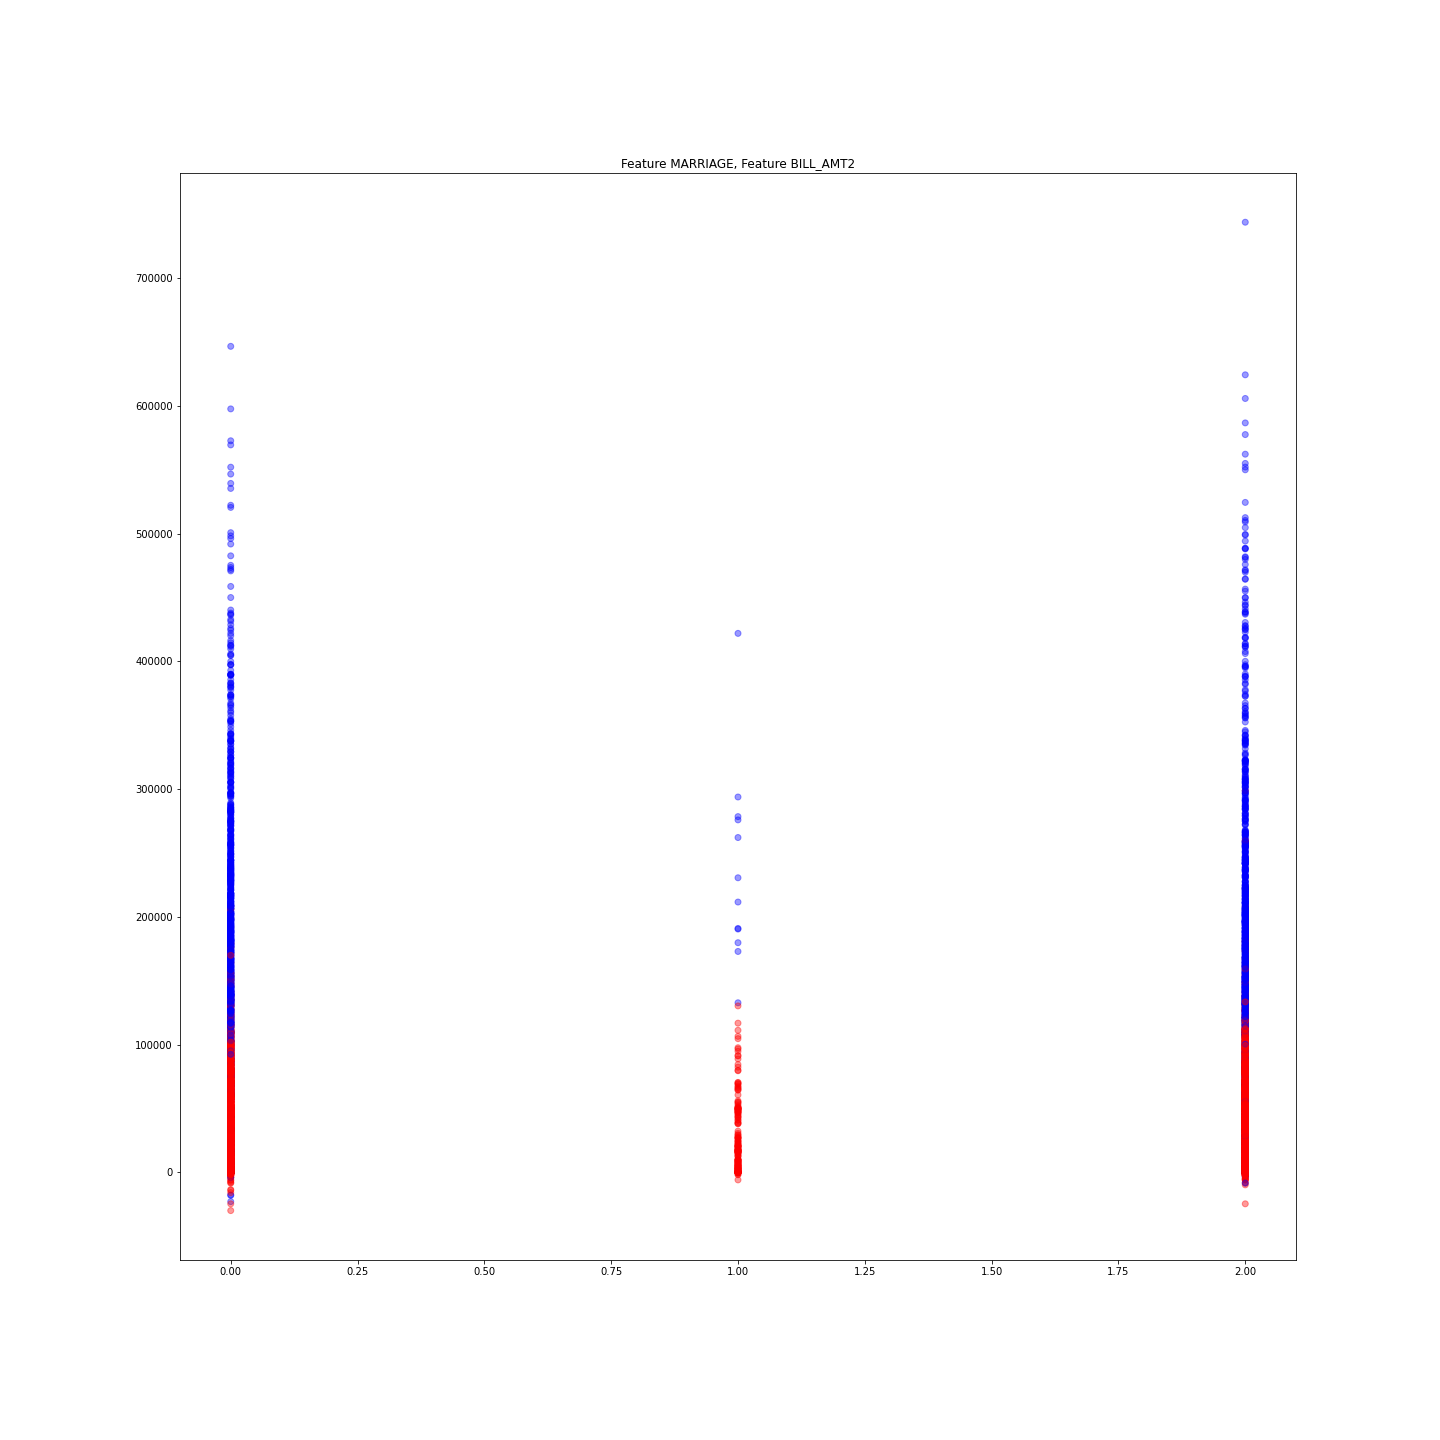
\includegraphics[width=\linewidth]{./images/ds2/clustering/kmeans/marriagelimitbal2.png}
			\caption{Data set 2 -- X-axis: Marriage status (0: 'married', 1: 'other', 2: 'single') vs. Y-axis: Balance limit, Kmeans clustering}
			\label{fig:kmeansds2}
		\end{subfigure}
	\end{figure}
	\begin{figure}[ht]\ContinuedFloat
		\begin{subfigure}{.5\textwidth}
			\centering
			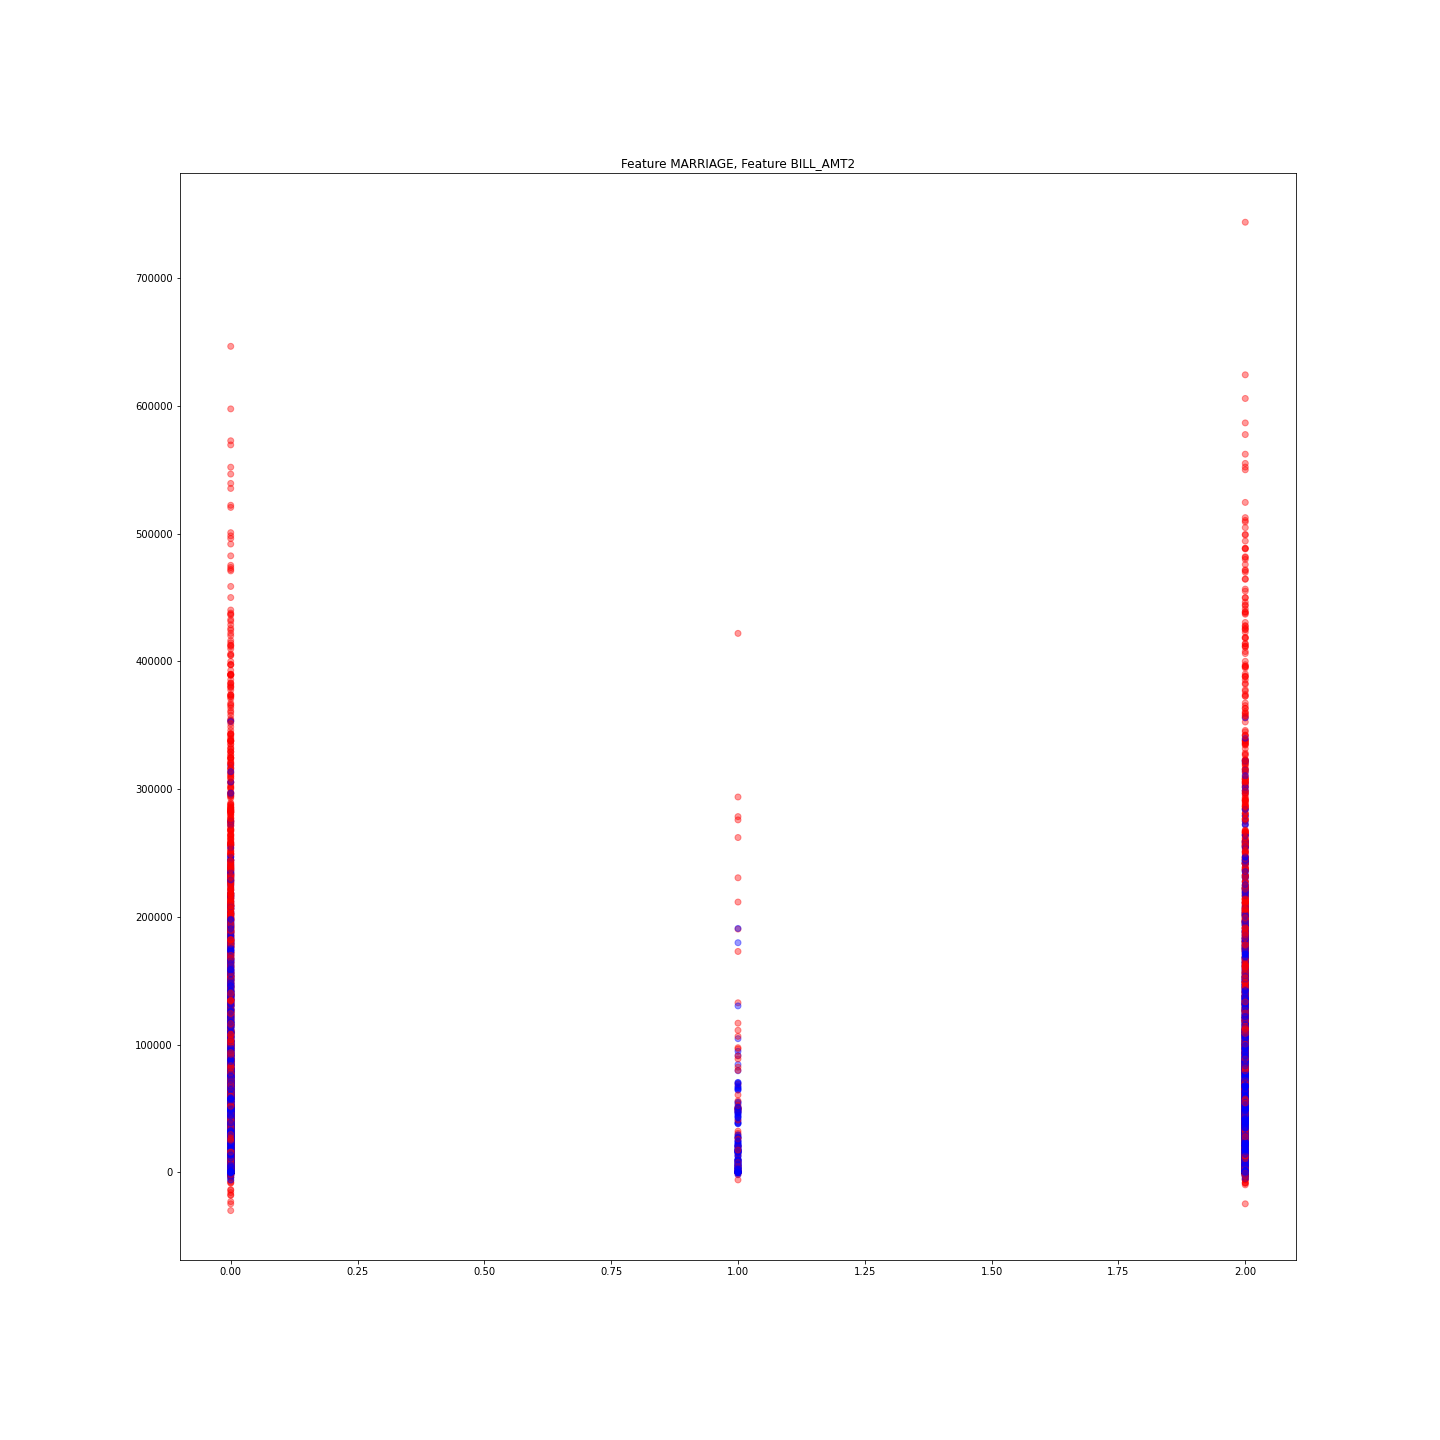
\includegraphics[width=\linewidth]{./images/ds2/clustering/kmeans/gmmarriagelimitbal2.png}
			\caption{Data set 2 -- X-axis: Marriage status (0: 'married', 1: 'other', 2: 'single') vs. Y-axis: Balance limit, Expectation maximization clustering}
			\label{fig:gmds2}
		\end{subfigure}
	\end{figure}
	\begin{figure}[ht]\ContinuedFloat
		\begin{subfigure}{.5\textwidth}
			\centering
			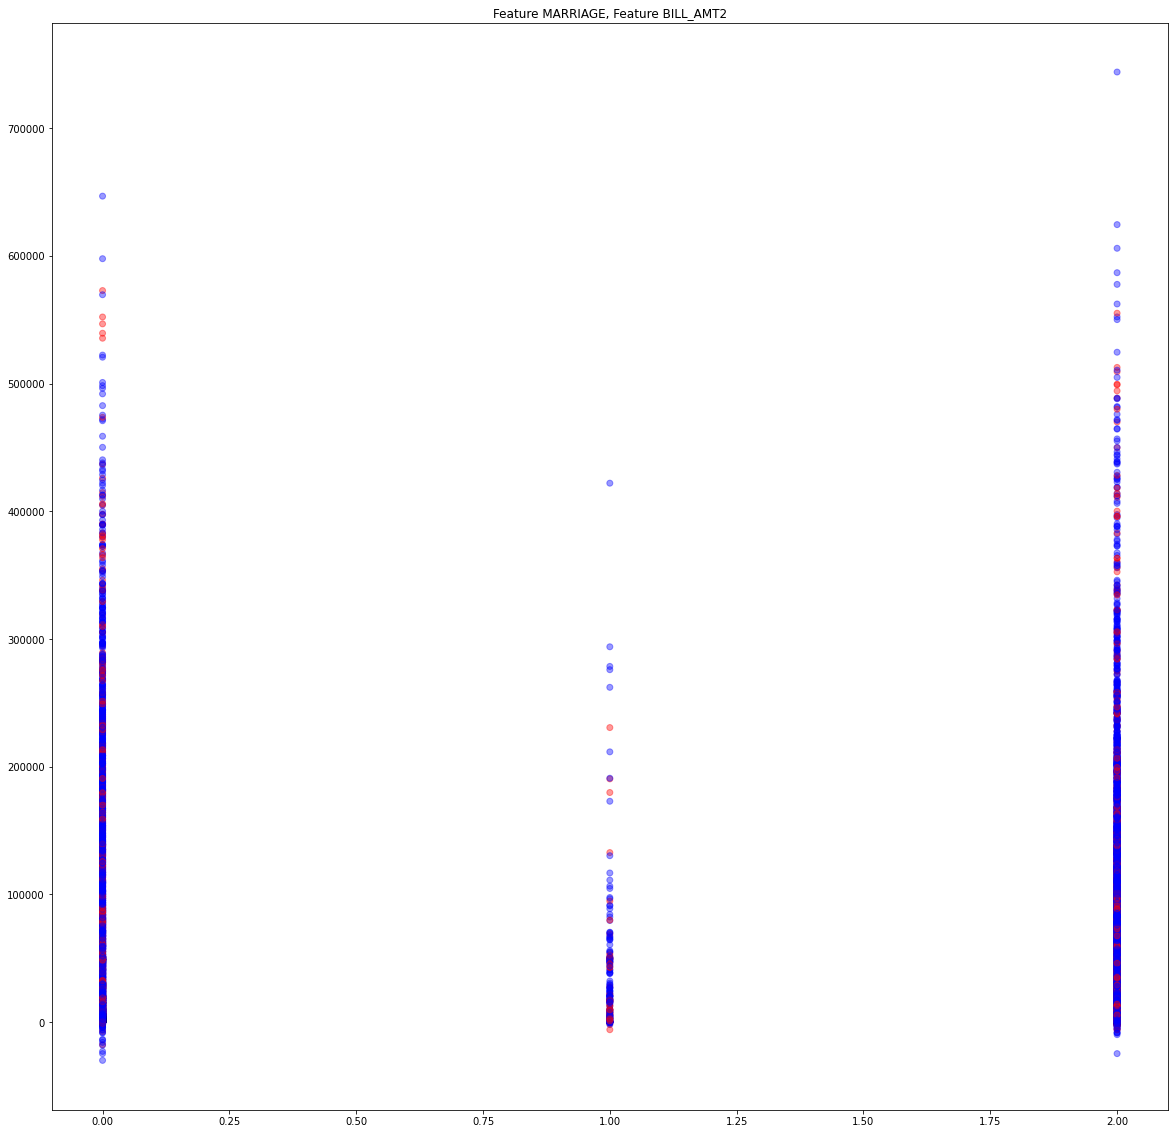
\includegraphics[width=\linewidth]{./images/ds2/clustering/kmeans/gtmarriagelimitbal2.png}
			\caption{Data set 2 -- X-axis: Marriage status (0: 'married', 1: 'other', 2: 'single') vs. Y-axis: Balance limit, Ground truth.}
			\label{fig:gtds2}
		\end{subfigure}
	\end{figure}

	For dataset 1, the clustering algorithms didn't provide much insight or useful information. This is mostly because of the number of discrete columns in the dataset, 3 continuous features for dataset 1 as compared to 13 for dataset 2, all though dataset 2's features I believe are mostly correlated (more exploration on this later in Dimensionality Reduction section).
	
	When looking at the dataset 2 clustering results shown in \cref{fig:kmeansds2,fig:gmds2,fig:gtds2}, in the ground truth image (\ref{fig:gtds2}) the output classes are more evenly distributed among the dataset for the features, Marriage status, and Balance limit. While the other two algorithms show a more clear distinct line of grouping the classes. What is interesting is how kmeans vs expectation maximization (EM) work to classify clusters. Kmeans claims points near its centers in a particular cluster, so in essence it draws a more hard line division between clusters, and we can see that in figure \ref{fig:kmeansds2}, where any bill amount above 100,000 is classified into the blue cluster. While in figure \ref{fig:gmds2} we can see a more varied mix of clusters in the middle of the data but tend to converge closer to a cluster at the extremes. This is because EM allows for points to be considered in either cluster based off the probability of that data point existing in the cluster. While the labels created by the clustering algorithm make sense in a common sense way, where the higher the credit balance for an individual the more likely they are to default on their loan. The reality shown in the ground truth scatter plot, figure \ref*{fig:gtds2} reveals that this is not as cut and dry.

	\section{Dimensionality Reduction}
	Dimensionality reduction is a subset of unsupervised machine learning algorithms which attempt to address the 'curse of dimensionality'. The curse of dimensionality states that as you add a new dimension (feature) to your data, the number of data points you need to learn on that data increases exponentially. However the hard part of reducing features is trying to determine what features maybe useful. This is where these class of algorithms come into use.
	
	\subsection{Experiments}
	In this part of the paper we will look at reducing the dimensions of our data using each of the following three algorithms, Principal Component Analysis, Independent component analysis, Random projections, and finally TODO. Experiments I ran were to run component reduction into each algorithm for various values of $N=[2, 13]$ for the number of components. From there I choose a random component value of 2 to compare each algorithm against using kmeans clustering. Finally using the newly reduced data, I trained a neural network with various architectures to optimize for accuracy. We will compare that data against training the original data on a neural network.
	
	\subsection{Principal Component Analysis - PCA}
	Principal component analysis is an algorithm which attempts to find lower dimensional data while still preserving the variance in the data. This is done by first calculating the first principal component which is a vector in the direction of maximal variance. The remaining $i -1$ components are all orthogonal to each other. This allows for reconstructing the data with the lowest l2 error. 
	\subsubsection{Clustering Reduced Data}
	\begin{figure}[!b]
		\begin{subfigure}{1.0\linewidth}
			\centering
			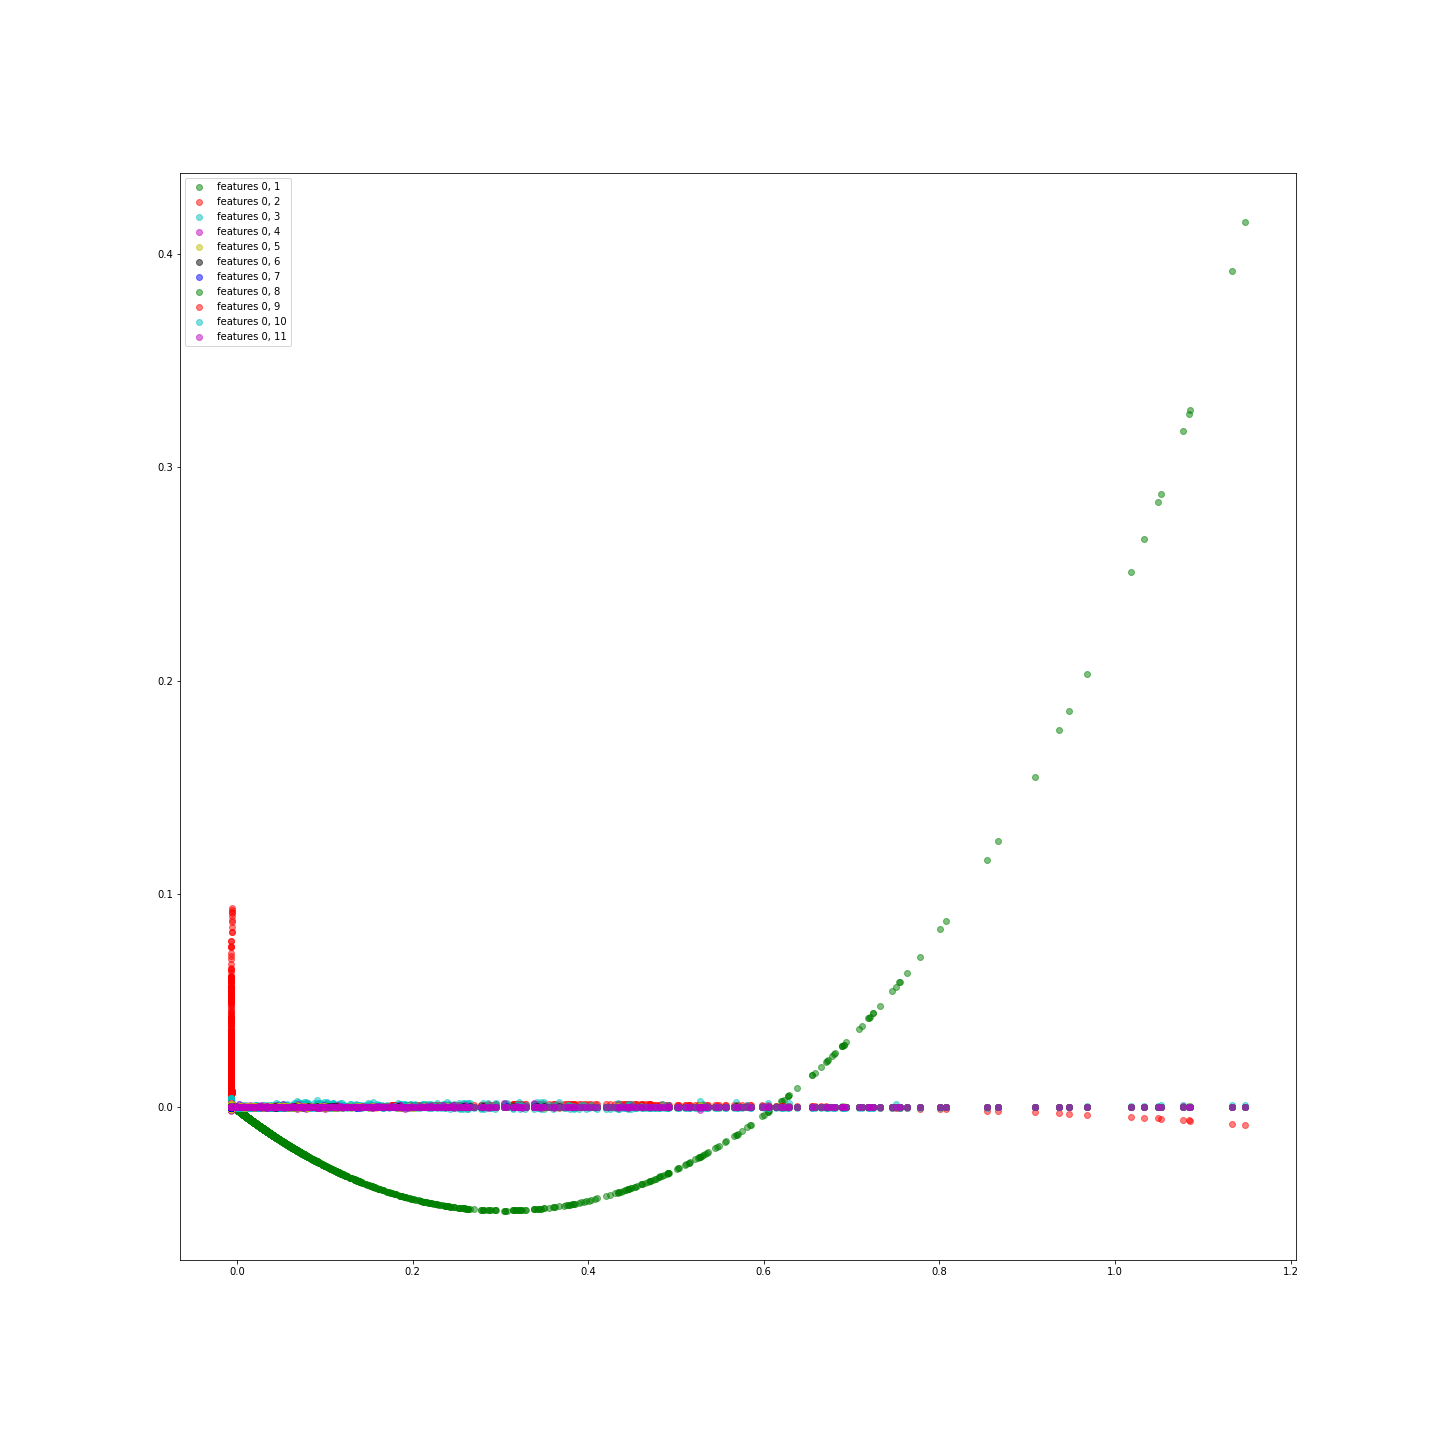
\includegraphics[width=\linewidth]{./images/ds1/pca/scatter/12components.png}
			\caption{Data set 1 -- PCA transformation values for component 0 plotted against other components.}
			\label{fig:pcads1scatter}
		\end{subfigure}
	\end{figure}
	\begin{figure}[ht]\ContinuedFloat
		\begin{subfigure}{.5\textwidth}
			\centering
			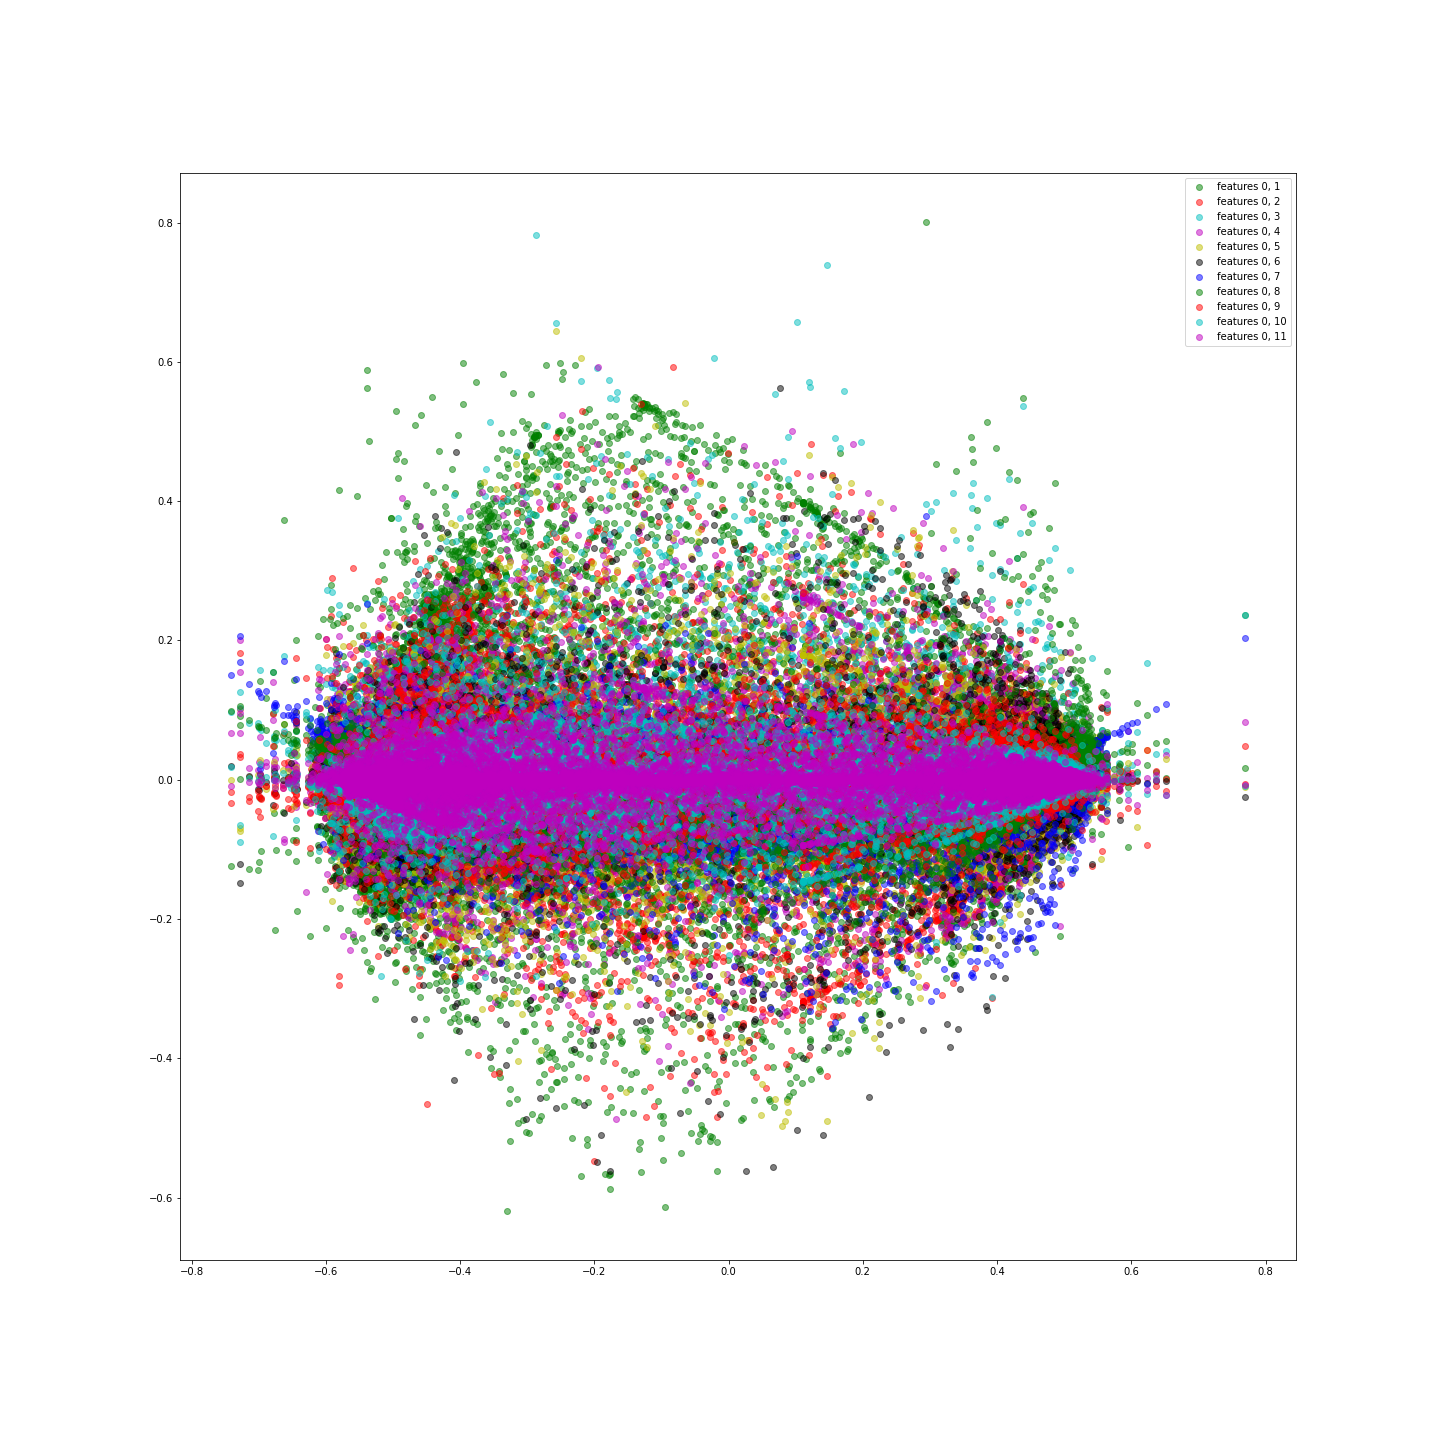
\includegraphics[width=\linewidth]{./images/ds2/pca/scatter/12components.png}
			\caption{Data set 2 -- PCA transformation values for component 0 plotted against other components.}
			\label{fig:pcads2scatter}
		\end{subfigure}
	\end{figure}
	\begin{figure}[ht]\ContinuedFloat
		\begin{subfigure}{.5\textwidth}
			\centering
			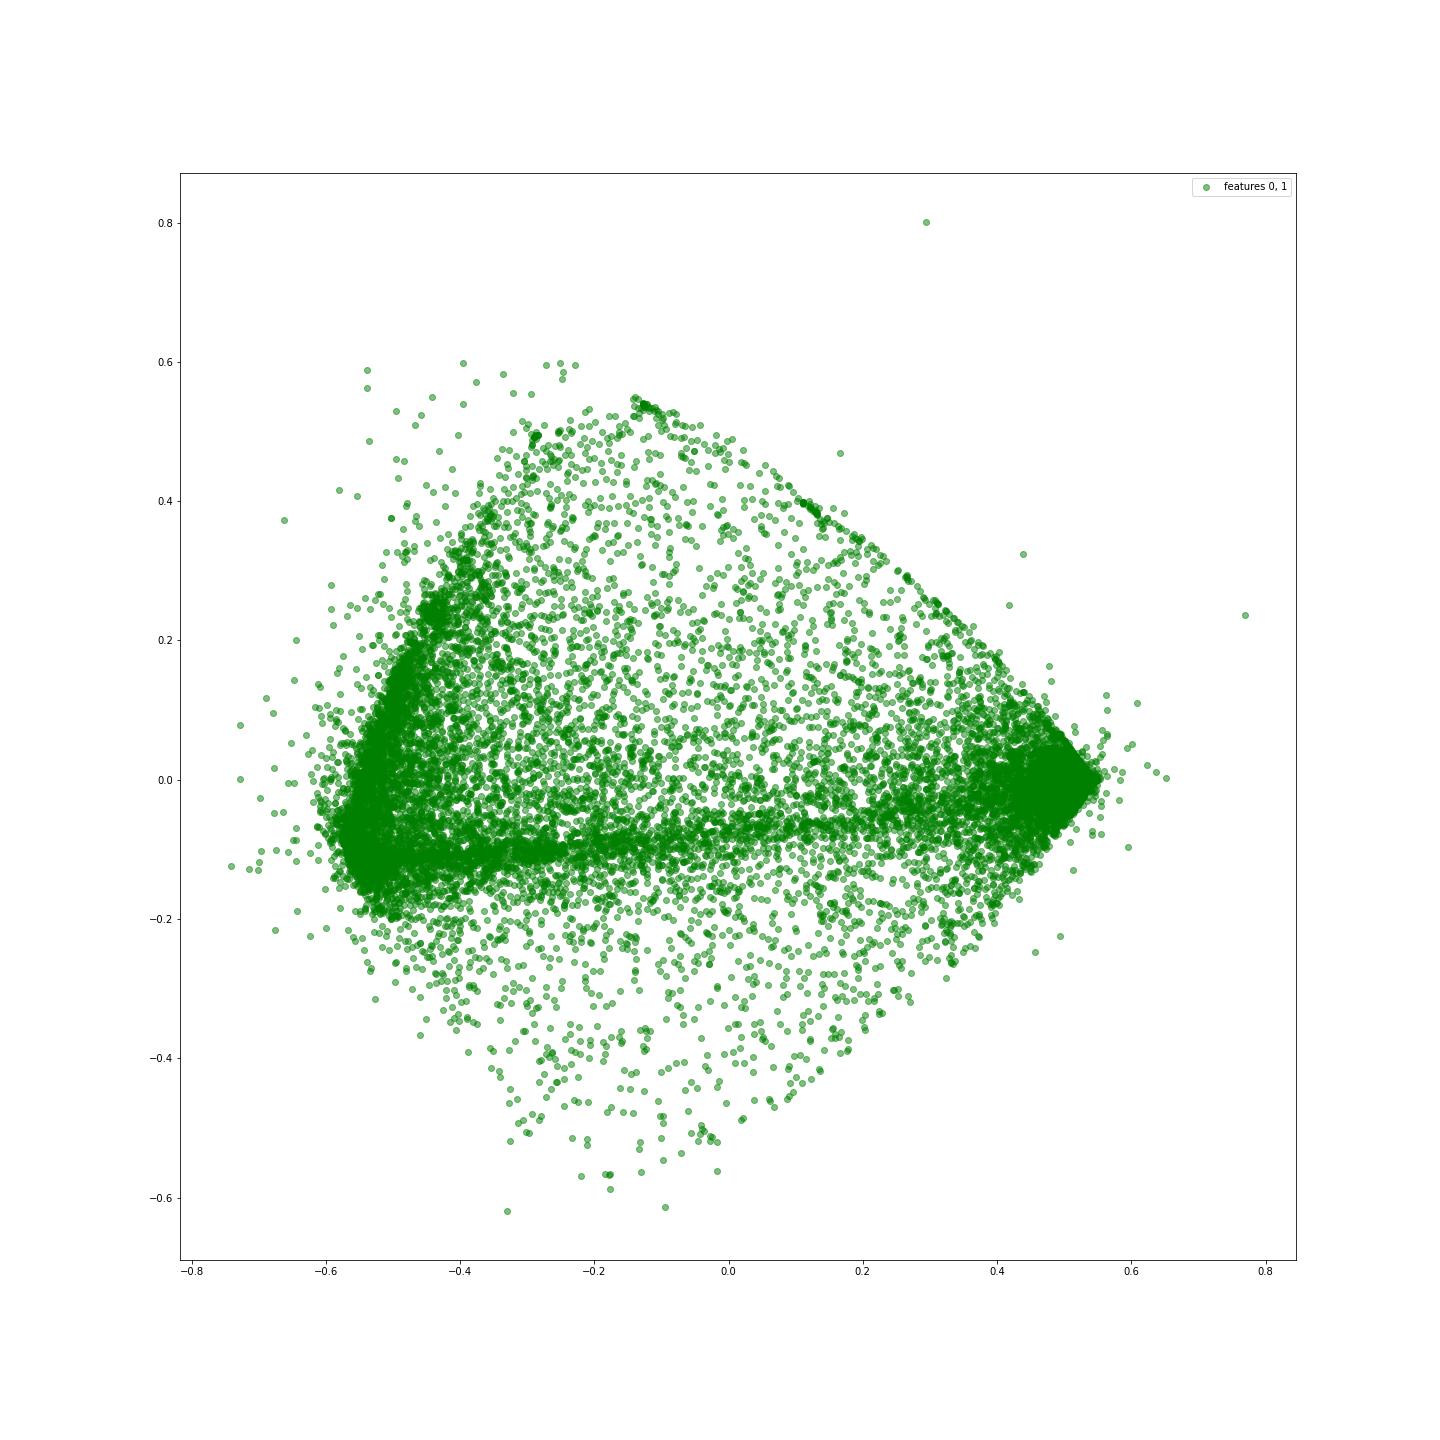
\includegraphics[width=\linewidth]{./images/ds2/pca/scatter/2components.png}
			\caption{Data set 2 -- PCA transformation for only 2 components}
			\label{fig:pcads2comp2}
		\end{subfigure}
	\end{figure}

	After running PCA for various values of $N$ components and plotting against various component features. We can see in \cref{fig:pcads1scatter,fig:pcads2scatter} how as the component value is increased the variance on the graph decreases. This is especially prevalent in figure \ref{fig:pcads2comp2}. We can see the variance of the green dots, compared more easily to the variance of the purple dogs in figure \ref{fig:pcads2scatter}. This makes sense as PCA will attempt to find the highest level of variance first, and as we add more components variance decreases. Looking back at data set 1 we can see that most of the variance lives in the first two components. This can be confirmed using scikit-learn PCA function with $n_components$ parameter set to 0.99 (runs PCA on various component amounts until variance accounts for 0.99). With the following code 
	
	\begin{lstlisting}
pca = PCA(n_components=0.99, 
	random_state=10)
pca.fit(X_train)
print(f'variance ratio 
	({pca.n_components_} components): 
	{pca.explained_variance_ratio_}')
	
>>> variance ratio 
	(2 components): 
	[0.9649001  0.02727739]
	\end{lstlisting}

	So we can see that to get 99\% variance we only need two components for dataset 1.
	
	\subsubsection{Kmeans clustering on reduced data}
	\begin{figure}[!b]
		\begin{subfigure}{1.0\linewidth}
			\centering
			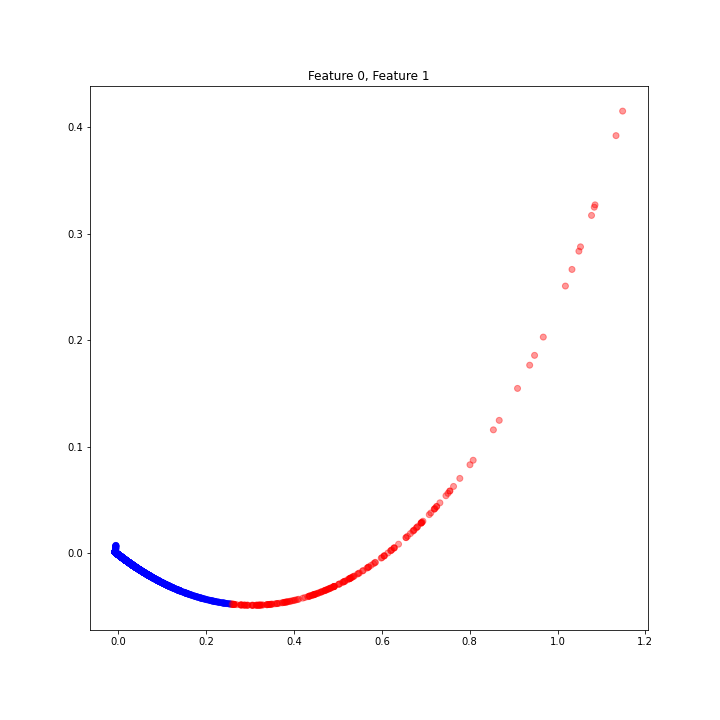
\includegraphics[width=\linewidth]{./images/ds1/pca/cluster/pcacluster.png}
			\caption{Data set 1 -- PCA transformation values for component = 2, and K=2 clusters, using K means.}
			\label{fig:pcads1cluster}
		\end{subfigure}
	\end{figure}
	\begin{figure}[ht]\ContinuedFloat
		\begin{subfigure}{0.5\textwidth}
			\centering
			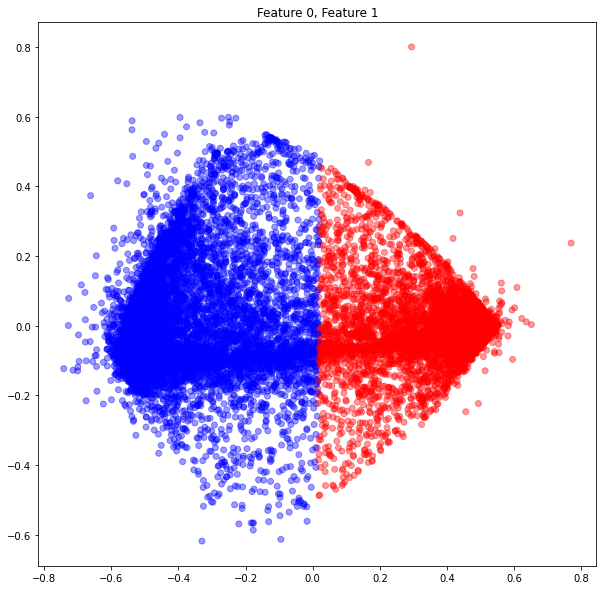
\includegraphics[width=\linewidth]{./images/ds2/pca/cluster/pcacluster.png}
			\caption{Data set 2 -- PCA transformation values for component = 2, and K=2 clusters, using K means}
			\label{fig:pcads2cluster}
		\end{subfigure}
	\end{figure}

	After reducing the data we can then see how kmeans clustering affects our clusters. Because each of the datasets are run to find 2 components using PCA we expect our data to look different that the original set of data, as is shown in the earlier figures for PCA as well as in \cref{fig:pcads1cluster,fig:pcads2cluster}. The benefit of using PCA though is that we can transform our data back to our original dataset with little error loss. using \lstinline|data_original = np.dot(data_reduced, pca.components_) + pca.mean_|, doing so gives us a l2 error of $1.316x10^-06$ for dataset one and $0.0015$ for dataset two. Which is pretty impressive taking dataset 1 down from, 14 features to 2, while dataset 2 is reduced further from 24 features to 2. The bad part about dimensionality reduction is we lose the link of the features to real world data. That is to say it is not easy to say what the two components of the datasets are composed of.

	\subsection{Independent Component Analysis - ICA}
	Independent component analysis like PCA and other algorithms here attempts to reduce the dimensionality of the data, but instead of finding the components of maximum variance, ICA will attempt to find a new set of features via linear transformation ($X \rightarrow Y$, where $X$ is the original set of features and $Y$ is the new set of features) in each each one of the new features are statistically independent of each other, or their mutual information is equal to 0, $I(y_i, y_j) =0$, and mutual information from $Y$ and $X$ is maximized.
	
	\subsubsection{Clustering Reduced Data}
	\begin{figure}[!b]
		\begin{subfigure}{1.0\linewidth}
			\centering
			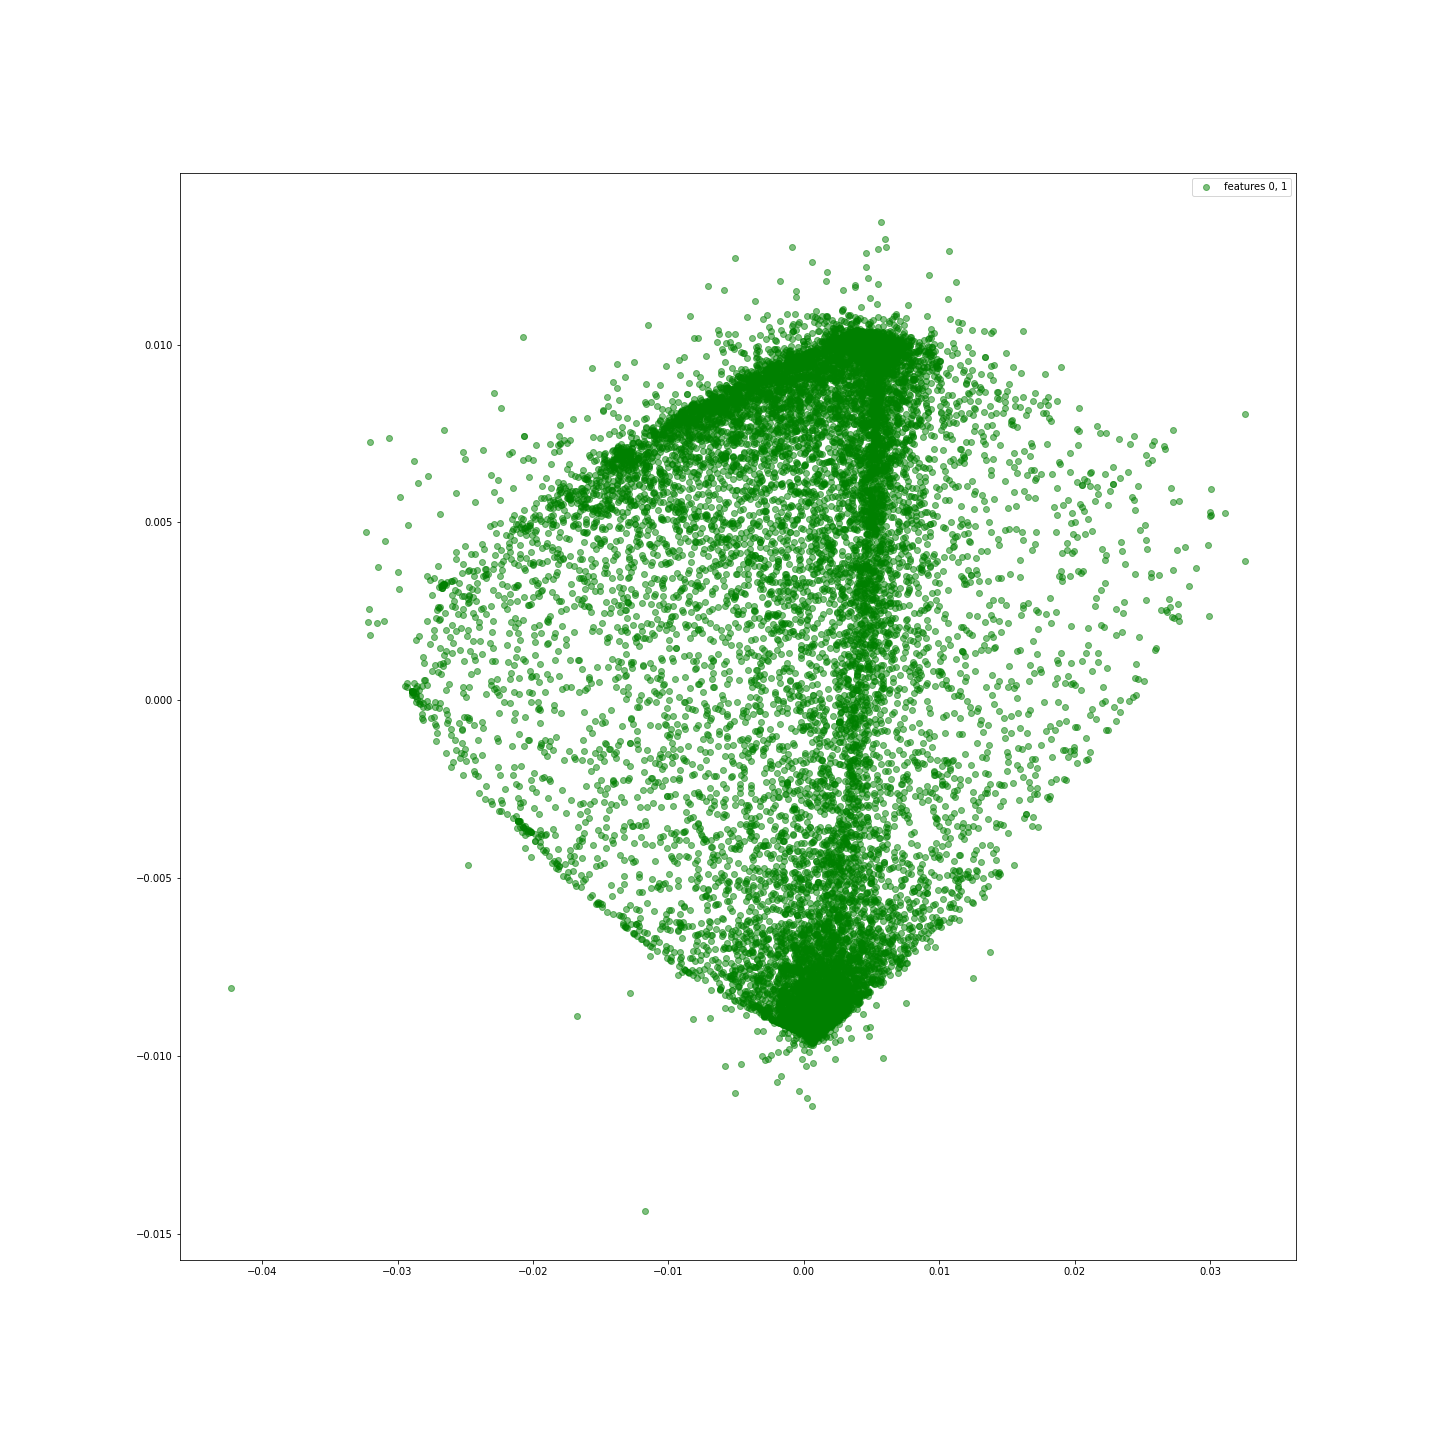
\includegraphics[width=\linewidth]{./images/ds2/ica/scatter/2components.png}
			\caption{Data set 2 -- ICA transformation for 2 components.}
			\label{fig:icads1scatter2}
		\end{subfigure}
	\end{figure}
	\begin{figure}[ht]\ContinuedFloat
		\begin{subfigure}{.5\textwidth}
			\centering
			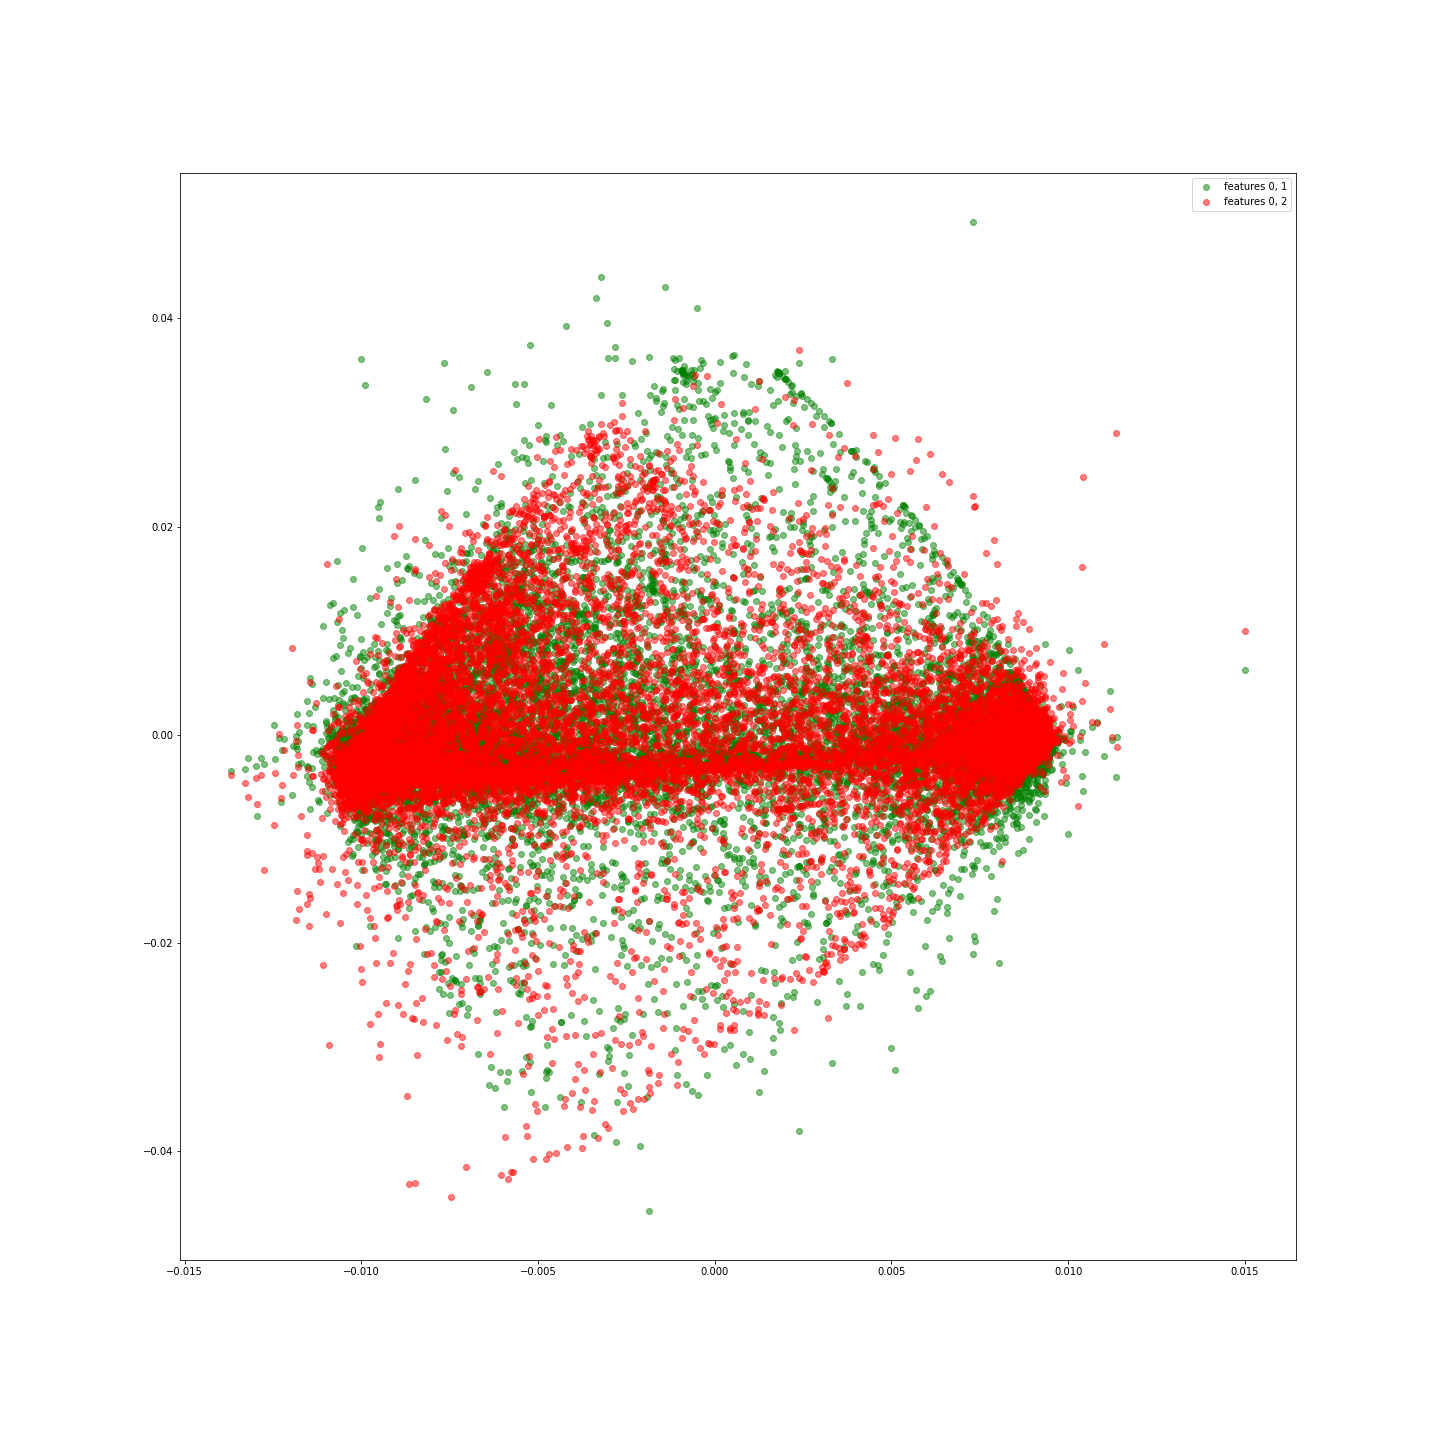
\includegraphics[width=\linewidth]{./images/ds2/ica/scatter/3components.png}
			\caption{Data set 2 -- ICA transformation for 3 components.}
			\label{fig:icads2scatter3}
		\end{subfigure}
	\end{figure}

	Similar to PCA reading the scatter plots for the dimensionally reduced data for ICA is very complicated. Because ICA attempts to find linearly independent features I noticed when looking through the plots especially for dataset 2. As I increased the number of components for ICA to use from run to run I would notice the data shift in a linear fashion. In the \cref{fig:icads1scatter2,fig:icads2scatter3}, we can see during the 2 component run the mass of scatter points running vertically down the center of the graph. While in the 3 component run the mass runs along the horizontal portion. While the change from the data has still made it unrecognizable, we can see between runs how it may use different linear combinations to reduce the data. 
	
	\subsection{Random Component Analysis - RCA}
	Random component analysis is different than the previous two algorithms, in the sense that those algorithms worked on some sort of foundation of mathematical functions. Random component analysis or random projection instead just takes the data and projects it into a random direction. While this approach may not do as well as PCA/ICA it still is effective at reducing the data needed by still maintaining the data correlation into lower dimensions. The advantage over this algorithm is the speed is much faster than the previous two algorithms.
	\subsubsection{Clustering Reduced Data}
	\begin{figure}[!b]
		\begin{subfigure}{1.0\linewidth}
			\centering
			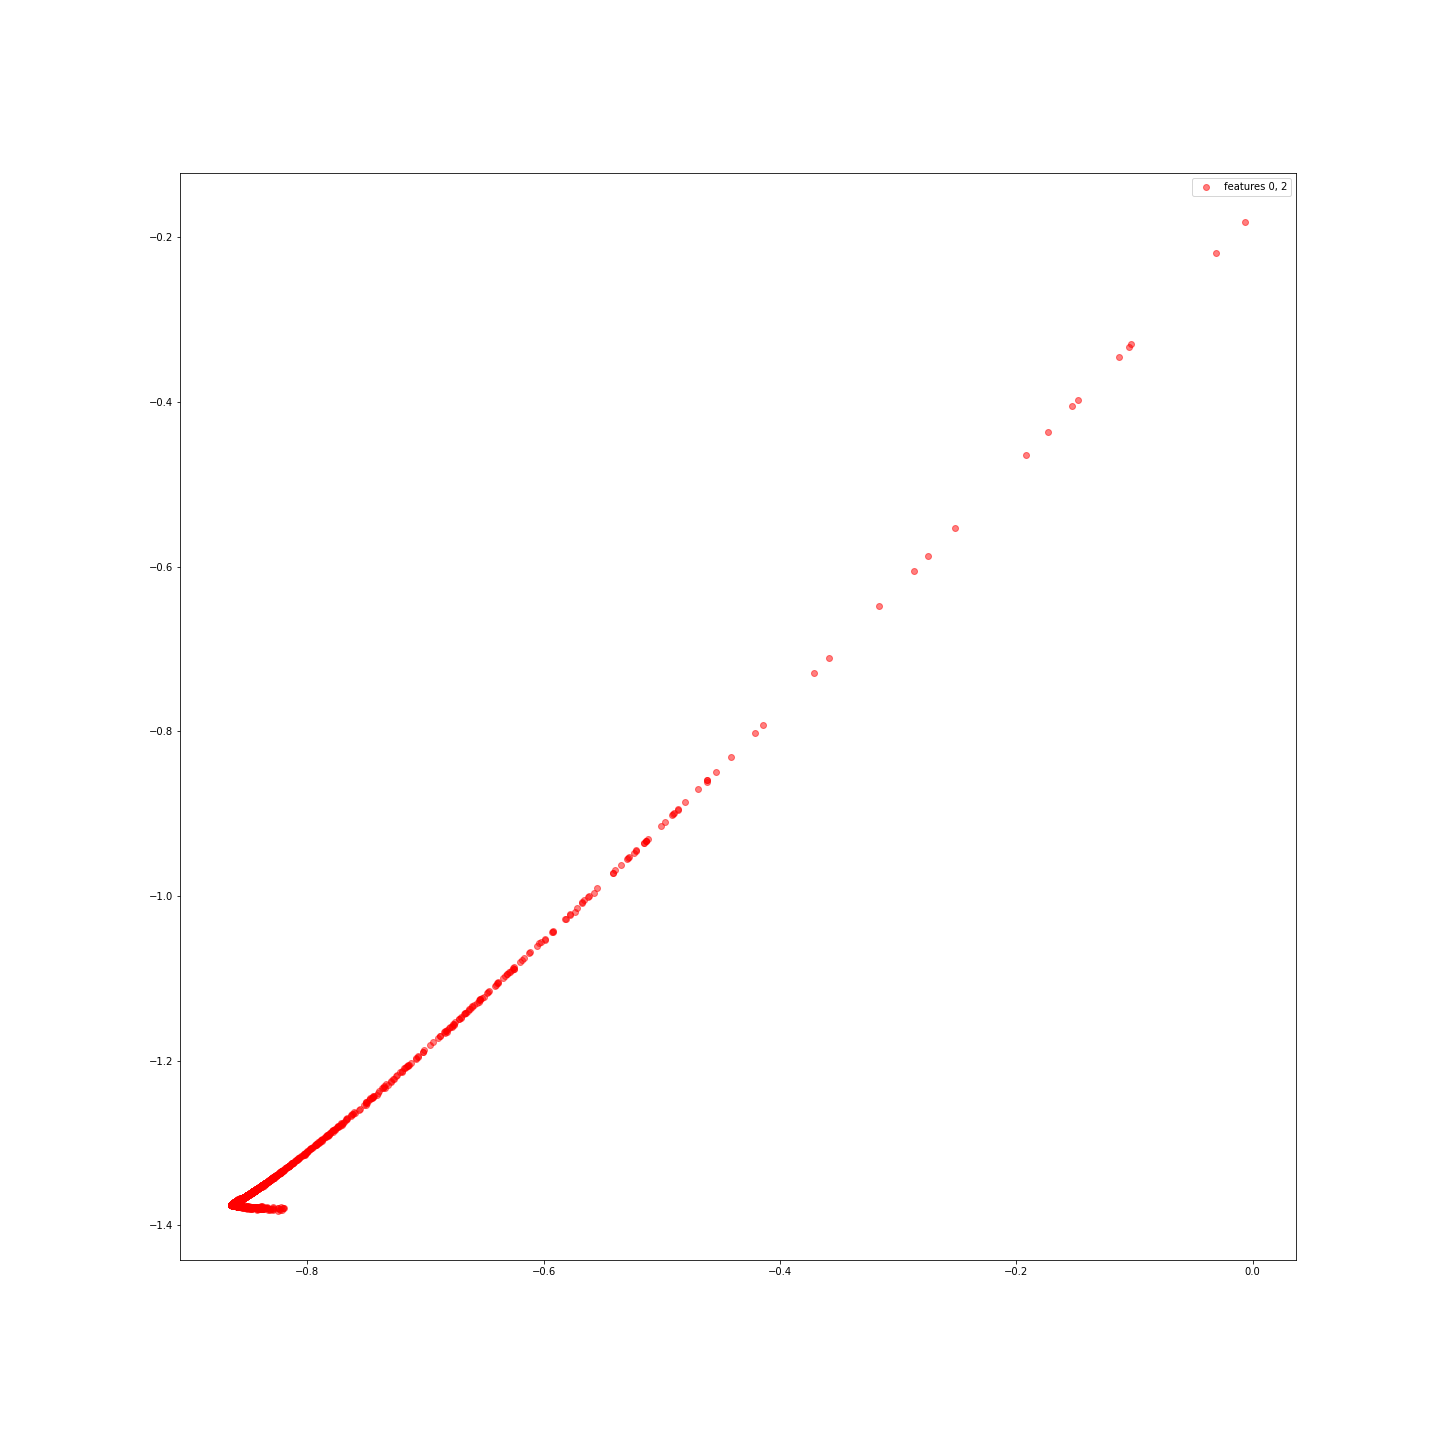
\includegraphics[width=\linewidth]{./images/ds1/rca/scatter/run1.png}
			\caption{Data set 1 -- RCA, with components = 2 run \#1.}
			\label{fig:rcarun1}
		\end{subfigure}
	\end{figure}
	\begin{figure}[ht]\ContinuedFloat
		\begin{subfigure}{.5\textwidth}
			\centering
			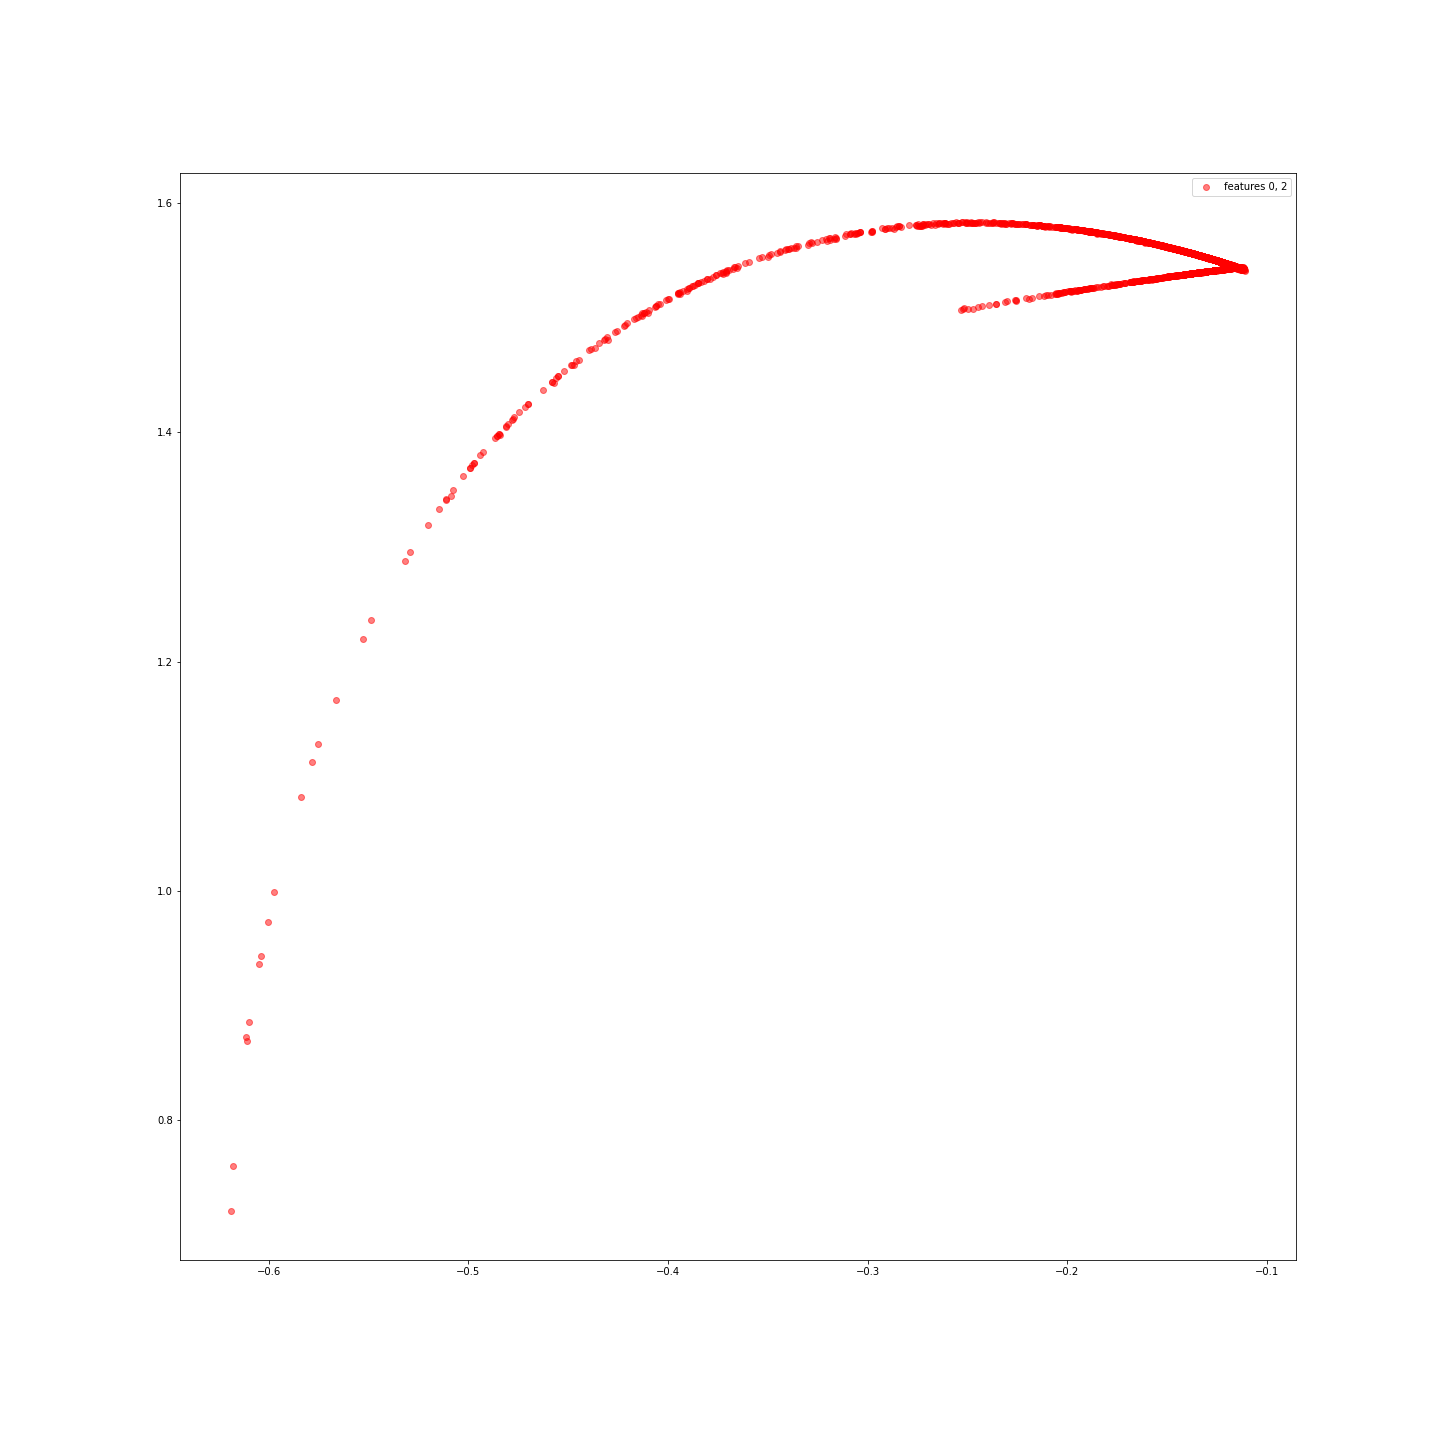
\includegraphics[width=\linewidth]{./images/ds1/rca/scatter/run2.png}
			\caption{Data set 1 -- RCA, with components = 2 run \#2.}
			\label{fig:rcarun2}
		\end{subfigure}
	\end{figure}
	\begin{figure}[ht]\ContinuedFloat
		\begin{subfigure}{.5\textwidth}
			\centering
			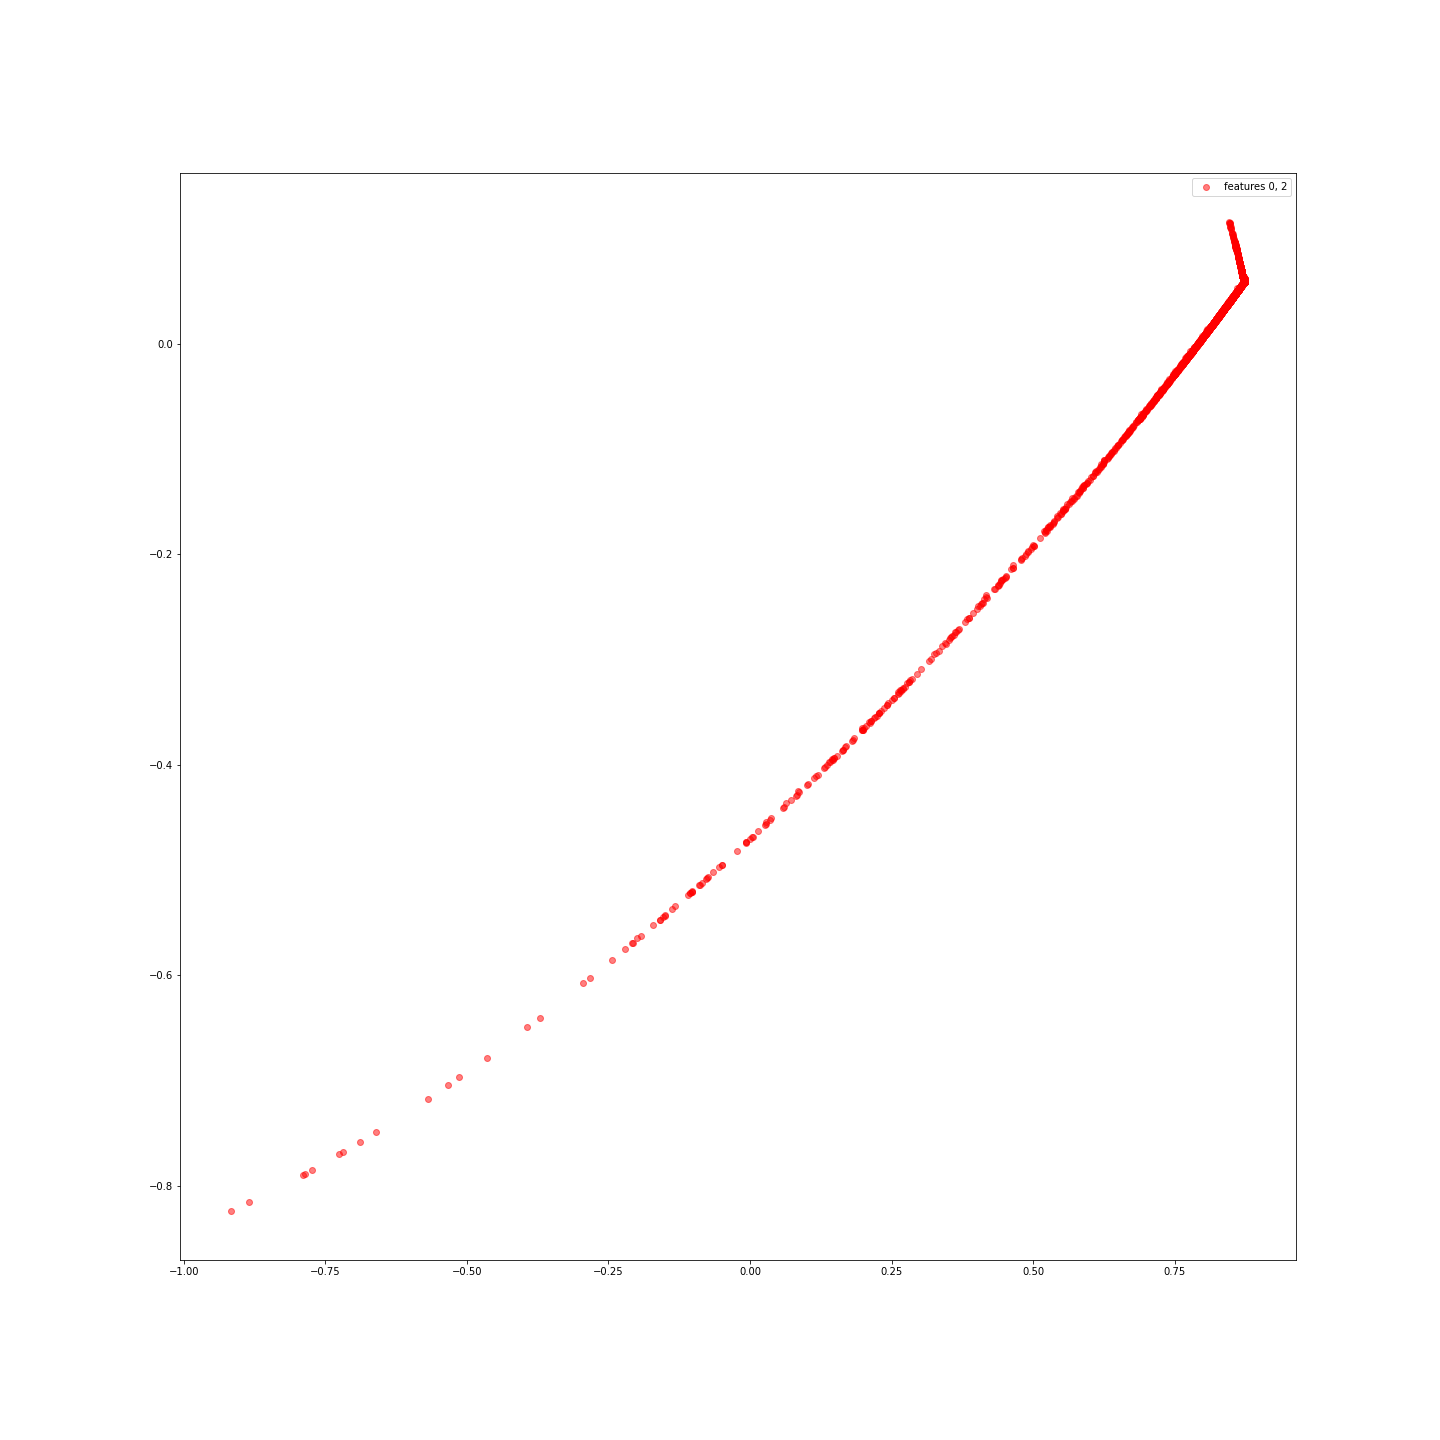
\includegraphics[width=\linewidth]{./images/ds1/rca/scatter/run3.png}
			\caption{Data set 1 -- RCA, with components = 2 run \#3.}
			\label{fig:rcarun3}
		\end{subfigure}
	\end{figure}
	Since RCA is randomly projecting data, analyzing the clustered data while useful may just have more results which look slightly more random than the two algorithms we have previously examined. As a result I have instead clustered 3 different runs of RCA with $n\_components=2$ to see how the algorithm returns back data. As we can see the results are vastly different from run to run, with no common pattern between the two.

	
	\subsection{Linear discriminant analysis - LDA}
	Last of our algorithms is Linear discriminant analysis (LDA) this algorithm attempts to find a projection that discriminates based on the label of the data. This is the only algorithm here which takes in the training labels in order to create the projection. This algorithm also has the constraint that $n_components<= min(n_classes - 1, n_features)$.
	\subsubsection{Clustering Reduced Data}
	\begin{figure}[!b]
		\begin{subfigure}{1.0\linewidth}
			\centering
			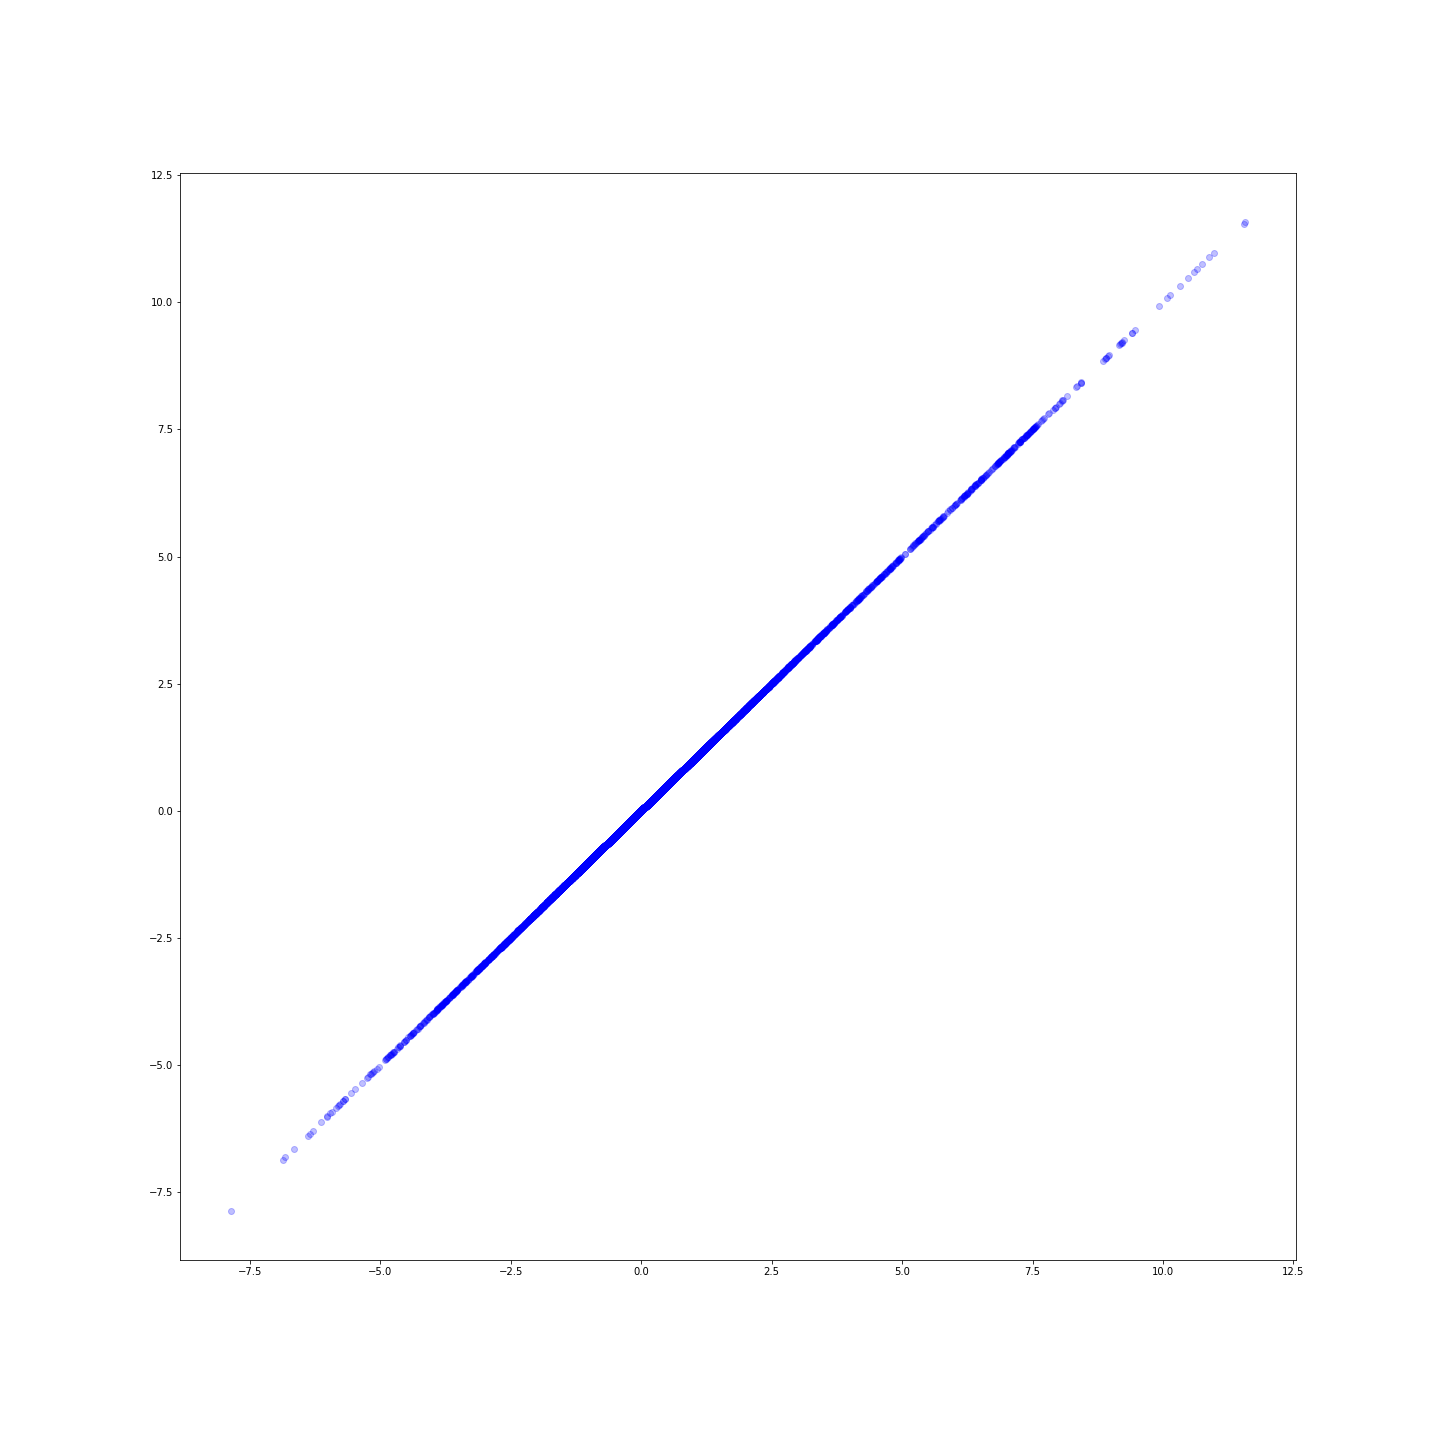
\includegraphics[width=\linewidth]{./images/ds1/lda/scatter.png}
			\caption{Data set 1 -- LDA, with components = 1 plotted against itself.}
			\label{fig:ldascatter}
		\end{subfigure}
	\end{figure}
	\begin{figure}[ht]\ContinuedFloat
		\begin{subfigure}{.5\textwidth}
			\centering
			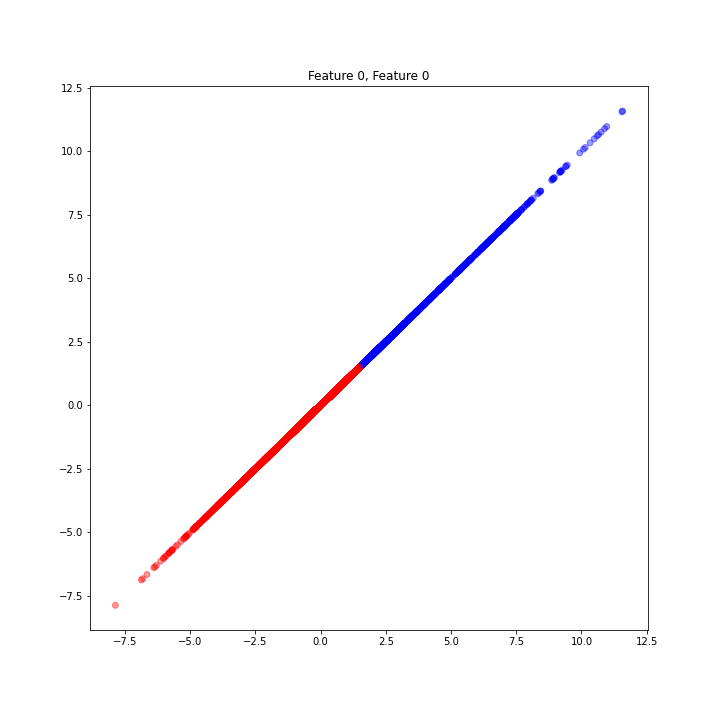
\includegraphics[width=\linewidth]{./images/ds1/lda/cluster.png}
			\caption{Data set 1 -- LDA, with components = 1 plotted against itself, using kmeans clustering.}
			\label{fig:ldacluster}
		\end{subfigure}
	\end{figure}
	
	Because LDA is a simple linear transformation based on the training data labels, the resulting graphs are straightforward for the two datasets, and as a result only dataset 1 is shown. The output is a single 1 dimensional array of values. We can see those values plotted against itself in \cref{fig:ldascatter,fig:ldacluster}. For running Kmeans clustering on the output we can see that the output divides the line pretty much down the middle, as expected.
	
	\subsection{Training a neural network on dimensionally reduced data}
	Neural networks are notoriously susceptible to needing large amounts of data to converge on its learning. By reducing the amount of input features to the neural network, ideally we should also be able to see some improvements both in terms of training time, and model accuracy. The results of this expierment are shown in \cref{fig:nnTestr,fig:nnTrain}, which shows the test accuracy of each neural network (architecture modeled best for the reduced dimensions). As well as the training time needed for the neural network to finished its learning respectively. We can see from the graph in figure \ref{fig:nnTestr} that while none of the neural networks trained on the dimensionally reduced datasets did better the original neural network for dataset 1. This was allured to early, that this could possibly be due to the higher number of discrete features. We do see though that all of the dimensionally reduced datasets were closer in their accuracy to one another. However in dataset 2 we see a bigger advantage of using dimensionality reduction where we get up to a 4\% accuracy gain for LDA, but improvements overall for all the algorithms. The last interesting call out is that LDA is able to out perform all other algorithms, this maybe due to the inclusion of using the labels in the dimension reduction, in addition to the large number of training examples in each set could cause this algorithm to perform well. The other important aspect of reducing the dimensions of our data is the ability to possibly train the models faster. In figure \ref{fig:nnTrain} we can see the training times for each of the datasets by the algorithm we used to reduce the dimensions, compared to the baseline. All of the algorithms were able to train faster than our baseline dataset. No one algorithm stands out on the dataset however. We can see for dataset 1 that PCA is almost 3 times faster to train than the baseline, and about 2 times faster than the next closest algorithm, ICA. Where as in dataset 2 ICA is able to outperform the baseline by also 3 times. This shows that by reducing the complexity of our data we are able to get better more performance out of our models training time wise.	
	\begin{figure}[!b]
		\begin{subfigure}{1.0\linewidth}
			\centering
			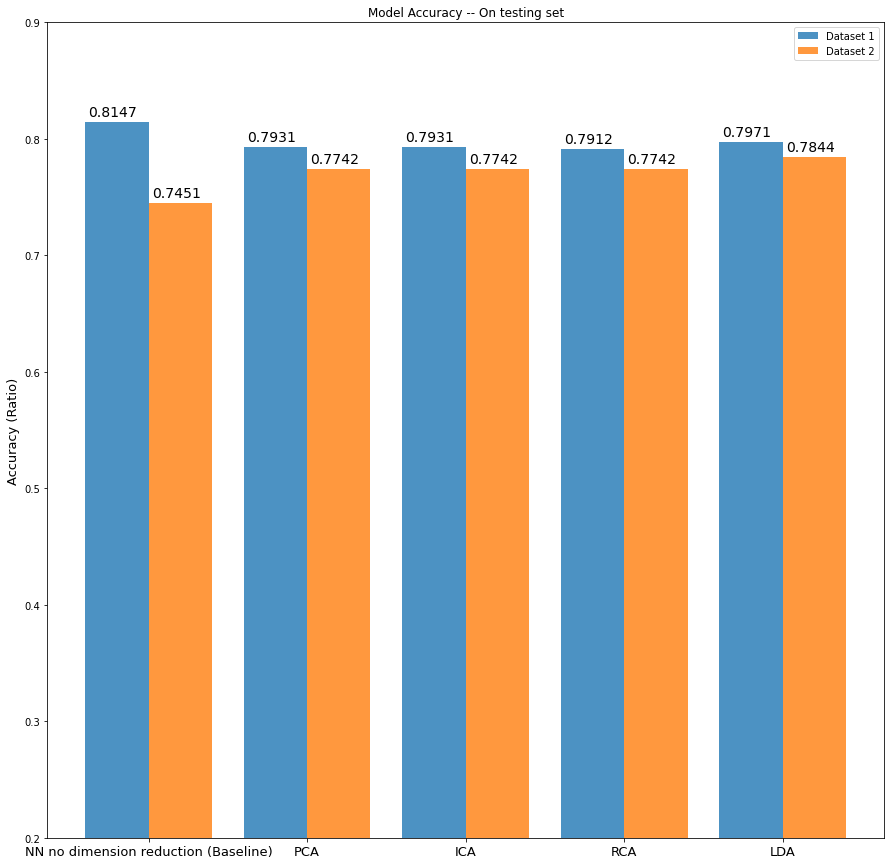
\includegraphics[width=\linewidth]{./images/nn/testAcc.png}
			\caption{Neural networks trained on no dimension reduction, PCA, ICA, RCA, and LDA -- various test accuracy for both dataset 1 and 2.}
			\label{fig:nnTestr}
		\end{subfigure}
	\end{figure}
	\begin{figure}[ht]\ContinuedFloat
		\begin{subfigure}{.5\textwidth}
			\centering
			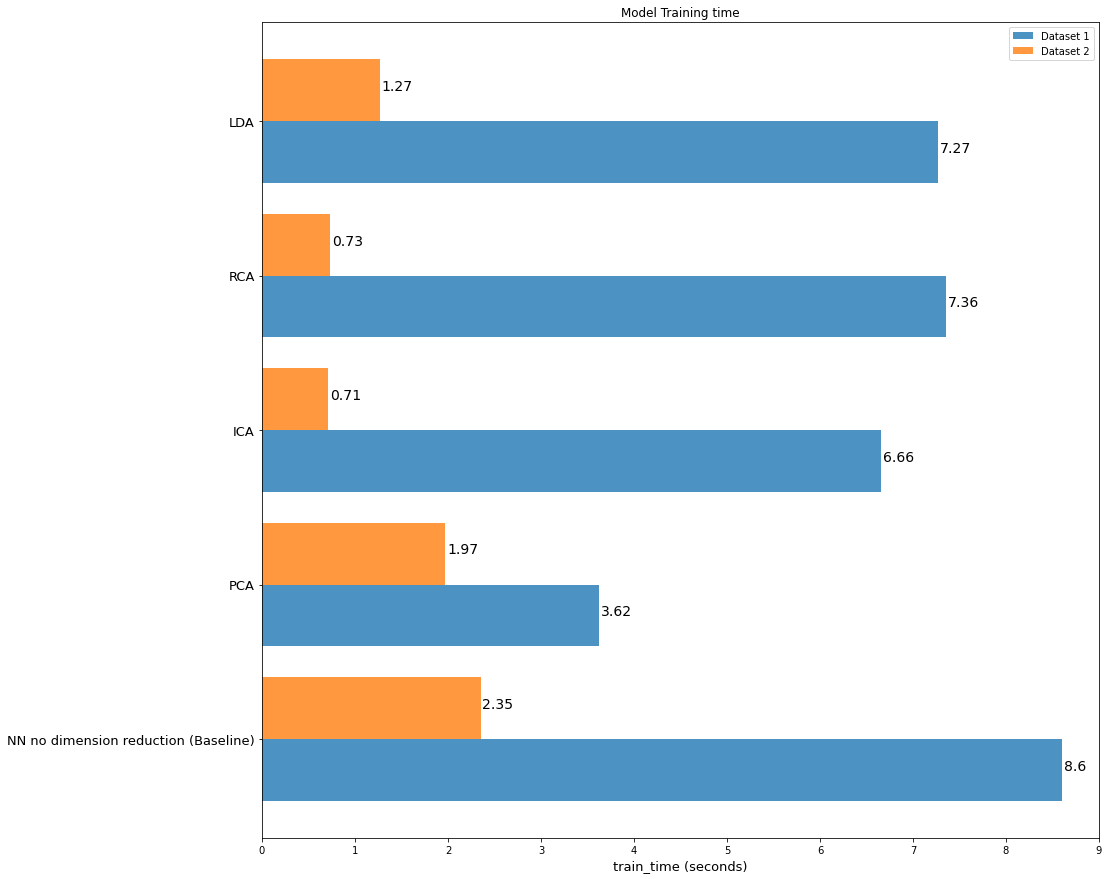
\includegraphics[width=\linewidth]{./images/nn/trainTime.png}
			\caption{Neural networks trained on no dimension reduction, PCA, ICA, RCA, and LDA -- various training time for both dataset 1 and 2.}
			\label{fig:nnTrain}
		\end{subfigure}
	\end{figure}
	
	\subsubsection{Adding clustering as a feature}
	Finally our last experiment is to see if we can use the output of clustering to help improve our neural networks by adding the cluster prediction as a feature in our dataset input to the neural network. Shown in \cref{fig:nnTestKmean,fig:nnTrainKmean} the results here are a more mixed bag that above. We can see some very slight performance in ICA and RCA for testing accuracy, up from 79.31\% accuracy to 79.57\% accuracy, and 79.12\% to 79.52\% respectively for dataset 1. This story again continues for training times, however we only see an improvement in RCA training time for dataset 1. This could possibly be attributed to better randomized components in the dimension reduction, as no other algorithms had a training time benefit.
	
	\begin{figure}[!b]
		\begin{subfigure}{1.0\linewidth}
			\centering
			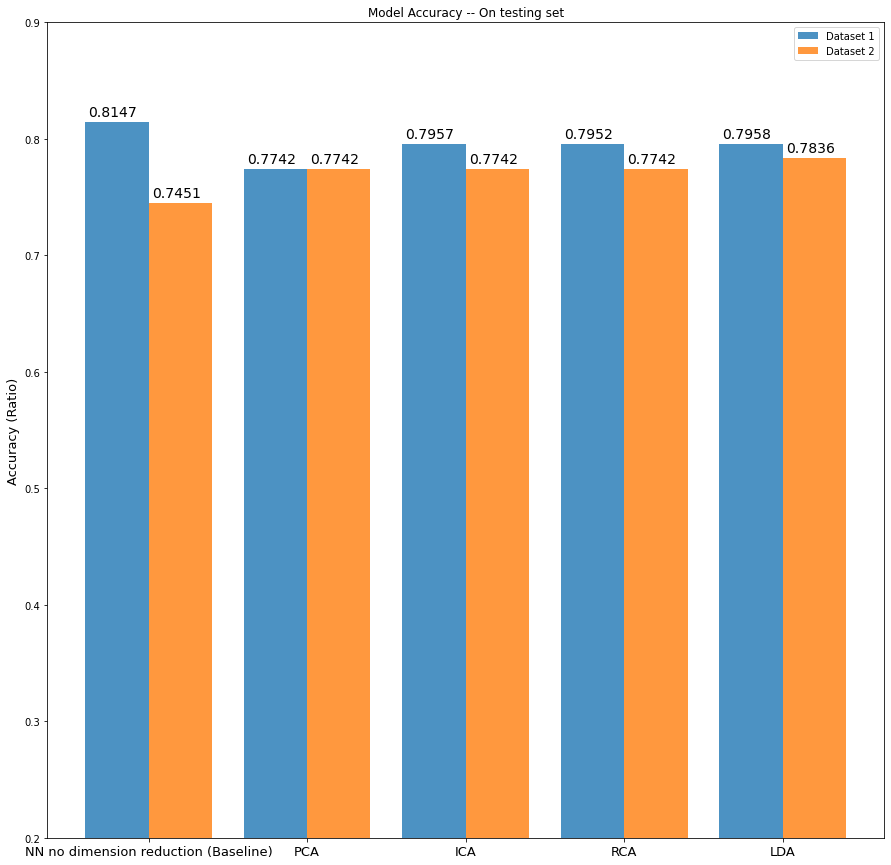
\includegraphics[width=\linewidth]{./images/nn/testAccKmean.png}
			\caption{Neural networks trained on no dimension reduction, PCA, ICA, RCA, and LDA -- various test accuracy for both dataset 1 and 2 with clustering feature.}
			\label{fig:nnTestKmean}
		\end{subfigure}
	\end{figure}
	\begin{figure}[ht]\ContinuedFloat
		\begin{subfigure}{.5\textwidth}
			\centering
			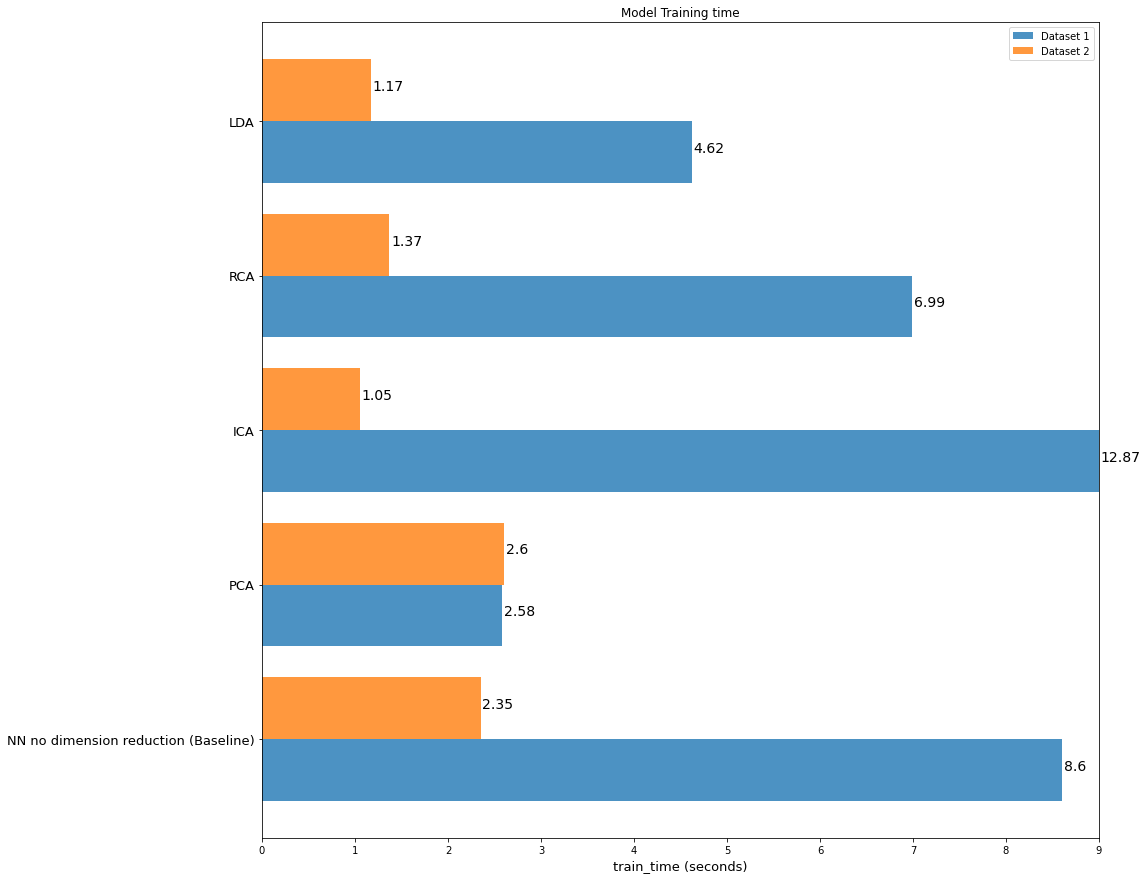
\includegraphics[width=\linewidth]{./images/nn/trainTimeKmean.png}
			\caption{Neural networks trained on no dimension reduction, PCA, ICA, RCA, and LDA -- various training time for both dataset 1 and 2 with clustering feature.}
			\label{fig:nnTrainKmean}
		\end{subfigure}
	\end{figure}

	\section{Conclusion}
	In this paper we looked at some common unsupervised learning algorithms. Two clustering algorithms used for data exploration. As we have learned understanding your data is key to getting the best results from your machine learning models. Clustering helps us visualize our data in new ways using computers to help us find possible patterns. Then we looked at how we can overcome the curse of dimensionality, which states that when a new feature is added to the dataset the number of examples needed to learn on the data goes up exponentially. Algorithms such as Principal component analysis, Independent component analysis, Random component analysis, and Linear discriminant analysis are all designed to project the data into a lower dimension feature space. We then took those algorithms and looked at how they can are used in practice. We saw that these algorithms aren't always a silver bullet to better results, but they can help in some cases. But in all cases reducing complexity of the data does improve training time.
	
	\nocite{*}
	\printbibliography[
	heading=bibintoc,
	title={References}
	] %Prints the entire bibliography with the title "Whole bibliography"
\end{document}\textsl{}